%\section{Figures}
\setcounter{figure}{0}
\setcounter{table}{0}
\renewcommand{\thefigure}{\arabic{figure}}
\renewcommand{\thetable}{\arabic{table}}
\begin{figure}
\figuretitle{Figure~\ref{fig:S173I_genetics_and_biochemistry}}
\begin{fullpanelvar}
    % What we would like to do here is incorporate the tex for the pedigree directly instead of using a standalone PDF.
    % \textbf{A}\\%
    % % \documentclass{standalone}
% %    \usepackage[landscape]{geometry}
%     \usepackage{pst-pdgr}
% \begin{document}

\newcommand{\heightgenone}{7}
\newcommand{\heightgentwo}{5}
\newcommand{\heightgenthree}{3}
\newcommand{\heightgenfour}{1}
\newcommand{\gensymbol}{0.5}

\newcommand{\heightlegenditemone}{8}
\newcommand{\heightlegenditemtwo}{7.25}
\newcommand{\heightlegenditemthree}{6.5}
\newcommand{\heightlegenditemfour}{5.75}
\newcommand{\legendleft}{9.25}

\begin{footnotesize}
\begin{pspicture}(22,9)
    \psset{descarmA=1.5, hatchsep=1.5pt}

    % Palpitations (7 family members total)
    %
    % Paternal uncle w/ palpitations, pursued workup (deceased of non-cardiac causes)
    \rput(5.25,\heightgentwo){\pstPerson[male, deceased, affected, belowtext=\parbox{2cm}{6}]{II6}}    
    % Mother of proband.
    \rput(13.25,\heightgentwo){\pstPerson[female, affected, belowtext=\parbox{2cm}{9}]{II9}}
    % Twin T
    \rput(7,\heightgenthree){\pstPerson[female, affected, belowtext=\parbox{1cm}{6}]{III6}}
    % Twin J
    \rput(8,\heightgenthree){\pstPerson[female, affected, belowtext=\parbox{1cm}{7}]{III7}}
    % Proband
    \rput(10.125,\heightgenthree){\pstPerson[female, affected, proband, belowtext=\parbox{1cm}{ 8\\35 y}, abovetext=]{III8}}
    % Half-sister of proband
    \rput(16.375,\heightgenthree){\pstPerson[female, affected, belowtext=\parbox{1cm}{12}]{III12}}
    % Child of proband
    \rput(9.75,\heightgenfour){\pstPerson[male, affected, belowtextrp=t, belowtext=\parbox{1cm}{\centering 4}]{IV4}}
    % Legend item
    \rput(\legendleft,\heightlegenditemone){\pstPerson[male, affected, righttext=\parbox{1cm}{Palpitations}]{legendPalp}}

    % Early SCD
    %
    % Paternal grandfather of proband
    \def\affectedstyle{fillstyle=crosshatch}
    \rput(2.75,\heightgenone){\pstPerson[male, deceased, affected, belowtextrp=t, belowtext=\parbox{3cm}{\centering 1\\SCD at age 45\\(found deceased)}]{I1}}
    % Also SIDS in generation IV, but not including this.
    % Legend item
    \rput(\legendleft,\heightlegenditemtwo){\pstPerson[male, affected, righttext=\parbox{2cm}{ SCD}]{legendSCD}}
    
    % SCD in the setting of other structural heart disease
    %
    \def\affectedstyle{fillstyle=vlines}
    % Father of proband.
    \rput(7,\heightgentwo){\pstPerson[male, deceased, affected, belowtext=\parbox{5cm}{ 8\\SCD at age 49 (during\\ETT; h/o MI, CABG)}]{II8}}
    % Half-sibling of proband.
    \rput(18.125,\heightgenthree){\pstPerson[male, deceased, affected, belowtext=\parbox{2cm}{ 13\\SCD at age 40\\(h/o CHD)}]{III13}}
    % Legend item
    \rput(\legendleft,\heightlegenditemthree){\pstPerson[male, affected, righttext=\parbox{4cm}{  SCD in setting of known\\CAD or CHD}]{legendSCDOther}}

    \rput(4,8){Ireland}
    \rput(16.5,8){Spain/France}

    % Generation 1, Ireland side.
    \rput(\gensymbol,\heightgenone){\Huge I}
    \rput(5,\heightgenone){\pstPerson[female, deceased, normal, belowtextrp=t, belowtext=\parbox{2cm}{\centering 2}]{I2}}
    \pstRelationship[descentnode=I1I2]{I1}{I2}

    % Generation 1, Spain/France side.
    \rput(15.5,\heightgenone){\pstPerson[male, deceased, belowtextrp=t, belowtext=\parbox{2cm}{\centering 3}]{I3}}
    \rput(17.5,\heightgenone){\pstPerson[female, deceased, belowtextrp=t, belowtext=\parbox{2cm}{\centering 4}]{I4}}
    \pstRelationship[descentnode=I3I4]{I3}{I4}

    % Generation II, Ireland side.
    \rput(\gensymbol,\heightgentwo){\Huge II}
    \rput(1.5,\heightgentwo){\pstPerson[male, belowtextrp=t, belowtext=\parbox{2cm}{\centering 1}]{II1}}
    \pstDescent{I1I2}{II1}
    \rput(2.25,\heightgentwo){\pstPerson[male, deceased, belowtext=\parbox{1cm}{2}]{II2}}    
    \pstDescent{I1I2}{II2}
    \rput(3,\heightgentwo){\pstPerson[male, deceased, belowtextrp=t, belowtext=\parbox{2cm}{\centering 3}]{II3}}    
    \pstDescent{I1I2}{II3}
    \rput(3.75,\heightgentwo){\pstPerson[male, deceased, belowtext=\parbox{2cm}{4}]{II4}}    
    \pstDescent{I1I2}{II4}
    \rput(4.5,\heightgentwo){\pstPerson[male, deceased, belowtextrp=t, belowtext=\parbox{2cm}{\centering 5}]{II5}}    
    \pstDescent{I1I2}{II5}
    \pstDescent{I1I2}{II6}
    \rput(6,\heightgentwo){\pstPerson[female, belowtext=\parbox{2cm}{7}]{II7}}
    \pstDescent{I1I2}{II7}
    \pstDescent{I1I2}{II8}

    % Generation II, Spain/France side.
    \pstRelationship[broken, descentnode=II8II9]{II8}{II9}
    \pstDescent{I3I4}{II9}

    \rput(18.5,\heightgentwo){\pstPerson[male, belowtextrp=t, belowtext=\parbox{2cm}{\centering 10}]{II10}}
    \pstRelationship[broken, descentnode=II9II10]{II9}{II10}

    \rput(20,\heightgentwo){\pstPerson[male, deceased, belowtext=\parbox{2cm}{11}, hatchsep=3pt]{II11}}
    \pstDescent{I3I4}{II11}
    \rput(21,\heightgentwo){\pstPerson[abovetext=, female, belowtext=\parbox{2cm}{12}]{II12}}
    \pstDescent{I3I4}{II12}

    % Generation III, proband and her siblings, half-siblings, and cousins.
    % First, the cousins on the Ireland side. 
    \rput(\gensymbol,\heightgenthree){\Huge III}
    \rput(2.25,\heightgenthree){\pstPerson[insidetext=N, belowtextrp=t, belowtext=\parbox{1cm}{\centering 1}]{III1}}
    \pstDescent{II2}{III1}
    \rput(3.375,\heightgenthree){\pstPerson[female, deceased, belowtextrp=t, belowtext=\parbox{1cm}{\centering 2}, abovetext=]{III2}}
    \pstDescent{II4}{III2}
    \rput(4.125,\heightgenthree){\pstPerson[insidetext=N, belowtextrp=t, belowtext=\parbox{2cm}{\centering 3}]{III3}}
    \pstDescent{II4}{III3}
    \rput(5.25,\heightgenthree){\pstPerson[insidetext=N, belowtextrp=t, belowtext=\parbox{2cm}{\centering 4}]{III4}}
    \pstDescent{II6}{III4}
    \rput(6,\heightgenthree){\pstPerson[insidetext=N, belowtextrp=t, belowtext=\parbox{2cm}{\centering 5}]{III5}}
    \pstDescent{II7}{III5}

    % Proband and siblings.
    \rput(7.5,3){\pnode{Twins1}}
    \pstTwins[qzygotic]{II8II9}{Twins1}{III6}{III7}
    \pstDescent{II8II9}{III8}
    % Brother of proband, deceased of non-cardiac causes.
    \rput(12.25,\heightgenthree){\pstPerson[male, deceased, belowtext=\parbox{1cm}{9}]{III9}}
    \pstDescent{II8II9}{III9}

    % Half-sibling group 1.
    \rput(13.625,\heightgenthree){\pstPerson[female, belowtext=\parbox{1cm}{10}]{III10}}
    \pstDescent{II9}{III10}

    % Half-sibling group 2.
    \rput(15,\heightgenthree){\pstPerson[female, belowtext=\parbox{1cm}{11}]{III11}}
    \pstDescent{II9II10}{III11}
    \pstDescent{II9II10}{III12}
    \pstDescent{II9II10}{III13}

    % Cousins
    \rput(20,\heightgenthree){\pstPerson[insidetext=N, belowtextrp=t, belowtext=\parbox{1cm}{\centering 14}]{III14}}
    \pstDescent{II11}{III14}
    \rput(21,\heightgenthree){\pstPerson[insidetext=N, belowtextrp=t, belowtext=\parbox{1cm}{\centering 15}]{III15}}
    \pstDescent{II12}{III15}

    % Generation IV
    \rput(\gensymbol,\heightgenfour){\Huge IV}

    % Children of twins T and J
    \rput(7,\heightgenfour){\pstPerson[belowtextrp=t, belowtext=\parbox{1cm}{\centering 1}]{IV1}}
    \pstDescent{III6}{IV1}
    \rput(8,\heightgenfour){\pstPerson[belowtextrp=t, belowtext=\parbox{1cm}{\centering 2}]{IV2}}
    \pstDescent{III7}{IV2}

    % Children of proband.
    \rput(9,\heightgenfour){\pstPerson[female, belowtextrp=t, belowtext=\parbox{1cm}{\centering 3}]{IV3}}
    \pstDescent{III8}{IV3}
    \pstDescent{III8}{IV4}
    \rput(10.5,\heightgenfour){\pstPerson[male, belowtextrp=t, belowtext=\parbox{1cm}{\centering 5}]{IV5}}
    \pstDescent{III8}{IV5}
    \rput(11.25,\heightgenfour){\pstPerson[female, belowtextrp=t, belowtext=\parbox{1cm}{\centering 6}]{IV6}}
    \pstDescent{III8}{IV6}

    % Child of proband's brother
    \rput(12.25,\heightgenfour){\pstPerson[belowtextrp=t, belowtext=\parbox{1cm}{\centering 7}]{IV7}}
    \pstDescent{III9}{IV7}

    % Children of proband's half-sibling (group 1)
    \rput(13.25,\heightgenfour){\pstPerson[belowtextrp=t, belowtext=\parbox{1cm}{\centering 8}]{IV8}}
    \pstDescent{III10}{IV8}
    \rput(14,\heightgenfour){\pstPerson[female, deceased, belowtextrp=t, belowtext=\parbox{1cm}{\centering 9}]{IV9}}
    \pstDescent{III10}{IV9}

    % Children of proband's half-siblings (group 2)
    \rput(15,\heightgenfour){\pstPerson[belowtextrp=t, belowtext=\parbox{1cm}{\centering 10}]{IV10}}
    \pstDescent{III11}{IV10}
    \rput(16,\heightgenfour){\pstPerson[female, deceased, belowtextrp=t, belowtext=\parbox{2.5cm}{\centering 11\\SIDS}]{IV11}}
    \pstDescent{III12}{IV11}
    \rput(16.75,\heightgenfour){\pstPerson[belowtextrp=t, belowtext=\parbox{1cm}{\centering 12}]{IV12}}
    \pstDescent{III12}{IV12}
    \rput(17.75,\heightgenfour){\pstPerson[female, belowtextrp=t, belowtext=\parbox{1cm}{\centering 13}]{IV13}}
    \pstDescent{III13}{IV13}
    \rput(18.5,\heightgenfour){\pstPerson[male, belowtextrp=t, belowtext=\parbox{1cm}{\centering 14}]{IV14}}
    \pstDescent{III13}{IV14}
    
\end{pspicture}
\end{footnotesize}

% \end{document} 

    % But it is not easy to get PSTricks to do this, since it wants to write eps.
    % Complex workarounds are possible, but the appropriate solution is probably a different pedigree drawing package (tikz-based) altogether.
    % For now, just incorporate a standalone PDF.
    \textbf{\figurepanela}\\%
    \includegraphics[width=\linewidth,height=2.75in,keepaspectratio]{../results/pedigree_S173I/output/pedigree_S173I_standalone.pdf}
\end{fullpanelvar}
\hfill
\begin{fullpanelvar}
    \textbf{\figurepanelb}\\%
    \input{../results/assembly_kinetics/output/kinetics_CPVT_mutation_S173I_85mM_K.pgf}
\end{fullpanelvar}
\hspace*{1cm}
\begin{fullpanelvar}
    \textbf{\figurepanelc}\\%
    \input{../results/assembly_kinetics/output/kinetics_CPVT_mutation_K180R_85mM_K.pgf}
\end{fullpanelvar}
\rowspacersmall
\begin{fullpanelvar}
    \textbf{\figurepaneld}\\%
    \input{../results/assembly_kinetics/output/kinetics_CPVT_mutations_K180R_Mg.pgf}
\end{fullpanelvar}
\caption[Dominant cardiac calsequestrin disease mutations]{\textbf{\headingsubsectionone}. \figurepanelcaptiona Pedigree of a large extended family with the S173I mutation and a CPVT-like phenotype. CABG = coronary artery bypass graft; CAD = coronary artery disease; CHD = congenital heart disease; ETT = exercise treadmill test; MI = myocardial infarction; SCD = sudden cardiac death; SIDS = sudden infant death syndrome. \figurepanelcaptionb Multimerization kinetics of the S173I mutant observed using a turbidity assay after addition of \SI{1}{\milli\Molar} \ch{CaCl2} to purified protein (pH 7.4, \SI{20}{\milli\Molar} NaCl, \SI{85}{\milli\Molar} KCl). \figurepanelcaptionc Multimerization kinetics of the K180R mutant observed using a turbidity assay (same conditions as in \textbf{b}). \figurepanelcaptiond Multimerization kinetics of the K180R mutant observed using a turbidity assay (same conditions as in B, but with \SI{2}{\milli\Molar} \ch{MgCl2} added prior to calcium).}
\label{fig:S173I_genetics_and_biochemistry}
\end{figure}

\begin{figure}
\figuretitle{Figure~\ref{fig:filament_overview}}
\begin{fullpanelvar}
    \begin{emptypanel}{}
        \node(filament)[inner sep=0pt,below right]{\includegraphics[width=\linewidth,height=1.25in,keepaspectratio]{../results/filament_overview/output/overview_surface_cropped.png}};
        %
        \node(captionA)[inner sep=0pt,above left] at (filament.north west) {\normalsize\textbf{\figurepanela}};
        %
        \path (filament.south)++(-1,3.15) coordinate (filament_dimer_NW);
        \path (filament.south)++(1,1) coordinate (filament_dimer_SE);
        %
        \path (filament.south)++(-1,3.15) coordinate (filament_tetramer_NW);
        \path (filament.south)++(2.7,0.5) coordinate (filament_tetramer_SE);
        %
        \node(dimerrectfilament) [fit={(filament_dimer_NW) (filament_dimer_SE)}, dashedrectanglefit] {};
        %
        \node(dimer_dimer_rect_filament) [fit={(filament_tetramer_NW) (filament_tetramer_SE)}, dashedrectanglefit] {};
        %
        \node(filament_caption)[above, inner sep=7pt] at (filament.north) {Cardiac Calsequestrin Filament};
        %
        %
        %
        \node(dimer)[inner sep=0pt,right=1.5cm of filament]{\includegraphics[width=\linewidth,height=1.25in,keepaspectratio]{../results/filament_overview/output/overview_dimer_cropped.png}};
        %
        \node(dimerrect) [fit=(dimer), dashedrectanglefit] {};
        \node(dimer_caption)[above, inner sep=7pt] at (dimer.north) {Dimer};
        %        
        \node(dimer_chainAlabel)[above, inner sep=0pt] at ([shift={(-0.125cm,-0.6cm)}]dimer.south west) {Chain A};
        \draw[] ([shift={(0cm,0.125cm)}]dimer_chainAlabel.north) -- ([shift={(0.25cm,0.125cm)}]dimer.south west);
        %
        \node(dimer_chainBlabel)[above, inner sep=0pt] at ([shift={(0.125cm,-0.6cm)}]dimer.south east) {Chain B};
        \draw[] ([shift={(0cm,0.125cm)}]dimer_chainBlabel.north) -- ([shift={(-0.25cm,0.125cm)}]dimer.south east);
        % \path (dimer.south west)++(0,-0.5) coordinate (chainA);
        % \path (dimer.south east)++(0,-0.5) coordinate (chainB);
        % %
        % \node(chainAlabel) [above, inner sep=2pt, align=center] at (chainA) {Chain A};
        % \node(chainBlabel) [above, inner sep=2pt, align=center] at (chainB) {Chain B};
        % %
        %
        %
        \node(dimer_dimer)[inner sep=0pt,below=4.5cm of filament.west,anchor=west]{\includegraphics[width=\linewidth,height=1.5in,keepaspectratio]{../results/filament_overview/output/overview_tetramer_cropped.png}};
        %
        \node(dimer_dimer_rect) [fit=(dimer_dimer), dashedrectanglefit] {};
        %
        % \path (dimer_dimer.north east)++(0,0) coordinate (dimer_dimer_chainA);
        % \path (dimer_dimer.south east)++(0.75,1) coordinate (dimer_dimer_chainB);
        % \path (dimer_dimer.north)++(1.5,-0.5) coordinate (dimer_dimer_chainAprime);
        % \path (dimer_dimer.south east)++(0.75,1) coordinate (dimer_dimer_chainBprime);
        %
        % \node(dimer_dimer_chainAlabel)[above, inner sep=0pt] at ([shift={(-0.25cm,0.75cm)}]dimer_dimer.north west) {Chain A};
        % \draw[] ([shift={(0cm,-0.25cm)}]dimer_dimer_chainAlabel.south) -- ([shift={(0.25cm,-0.125cm)}]dimer_dimer.north west);
        % %
        % \node(dimer_dimer_chainBlabel)[above, inner sep=0pt] at ([shift={(-0.25cm,0.5cm)}]dimer_dimer.north) {Chain B};
        % \draw[] ([shift={(0cm,-0.25cm)}]dimer_dimer_chainBlabel.south) -- ([shift={(-0.25cm,-0.125cm)}]dimer_dimer.north);
        %
        \node(dimer_dimer_chainAprimelabel)[above, inner sep=2pt] at ([shift={(0.9cm,0.75cm)}]dimer_dimer.east) {Chain A'};
        \draw[] ([shift={(0cm,0cm)}]dimer_dimer_chainAprimelabel.west) -- ([shift={(-0.25cm,0.5cm)}]dimer_dimer.east);
        %
        \node(dimer_dimer_chainBprimelabel)[above, inner sep=2pt] at ([shift={(0.9cm,-0.5cm)}]dimer_dimer.south east) {Chain B'};
        \draw[] ([shift={(0cm,0cm)}]dimer_dimer_chainBprimelabel.west) -- ([shift={(-0.125cm,0.125cm)}]dimer_dimer.south east);
        % \node(dimer_dimer_chainAlabel) [above, inner sep=2pt, align=center] at (dimer_dimer_chainA) {Chain A};
        % \node(dimer_dimer_chainBlabel) [above, inner sep=2pt, align=center] at (dimer_dimer_chainB) {Chain B};
        % \node(dimer_dimer_chainAprimelabel) [above, inner sep=2pt, align=center] at (dimer_dimer_chainAprime) {Chain A'};
        % \node(dimer_dimer_chainBprimelabel) [above, inner sep=2pt, align=center] at (dimer_dimer_chainBprime) {Chain B'};
        %
        %
        %
        \path[-] (dimerrectfilament.east) edge (dimerrect.west);
        \path[-] (dimer_dimer_rect_filament.south) edge (dimer_dimer_rect.north);
        %
        % Beginning of thioredoxin stuff
        %
        \node(filament_thio)[inner sep=0pt,below=5cm of dimer_dimer.west,anchor=west]{\includegraphics[width=\linewidth,height=1.25in,keepaspectratio]{../results/filament_overview/output/overview_surface_thioredoxins_cropped.png}};
        %
        \node(captionA)[inner sep=0pt,above left] at (filament_thio.north west) {\normalsize\textbf{\figurepanelb}};
        %
        \path (filament_thio.south)++(-1,1.1) coordinate (thioprotomerSW);
        \path (filament_thio.south)++(1,3.1) coordinate (thioprotomerNE);
        %
        \node(protomerrectfilament) [fit={(thioprotomerSW) (thioprotomerNE)}, dashedrectanglefit] {};
        %
        \node(filament_caption)[above, inner sep=7pt] at (filament_thio.north) {Cardiac Calsequestrin Filament (Colored by Thioredoxin Domain)};
        %
        %
        %
        \node(monomers)[inner sep=0pt,right=1.5cm of filament_thio]{\includegraphics[width=\linewidth,height=1.25in,keepaspectratio]{../results/filament_overview/output/overview_monomers_cropped.png}};
        %
        \node(protomerrect) [fit={(monomers.south) (monomers.north west)}, dashedrectanglefit] {};
        %
        \node(domainI)[above, inner sep=0pt] at ([shift={(2cm,1cm)}]monomers.north) {Domain I};
        \draw[] ([shift={(0cm,-0.25cm)}]domainI.south) -- ([shift={(2.25cm,0.125cm)}]monomers.north);
        %
        \node(domainII)[below left, inner sep=0pt] at ([shift={(0.8cm,-0.8cm)}]monomers.south) {Domain II};
        \draw[] ([shift={(0cm,0.25cm)}]domainII.north) -- ([shift={(1cm,0.15cm)}]monomers.south);
        %
        \node(domainIII)[below left, inner sep=0pt] at ([shift={(0cm,-0.8cm)}]monomers.south east) {Domain III};
        \draw[] ([shift={(0cm,0.25cm)}]domainIII.north) -- ([shift={(-0.6cm,-0.2cm)}]monomers.south east);
        %
        %
        \path (monomers.north)++(-0.75,-1) coordinate (domains);
        %
        %
        %
        %
        \node(filament_thio_inner)[inner sep=0pt,below=4.5cm of filament_thio.west,anchor=west]{\includegraphics[width=\linewidth,height=1.25in,keepaspectratio]{../results/filament_overview/output/overview_surface_thioredoxins_23_domain_colors_cropped.png}};
        %
        \node(captionB)[inner sep=0pt,above left] at (filament_thio_inner.north west) {\normalsize\textbf{\figurepanelc}};
        %
        \node(filament_caption)[above, inner sep=7pt] at (filament_thio_inner.north) {Thioredoxin Domain II/III Double Helix};
        %
        %
        %
        \path[-] (protomerrect.north west) edge (protomerrectfilament.east);
        %    
    \end{emptypanel}
\end{fullpanelvar}
\caption[Overview of the cardiac calsequestrin filament]{\textbf{\headingsubsectiontwo}. \figurepanelcaptiona The cardiac calsequestrin candidate filament (PDB ID 6OWV) is shown, along with a representative dimeric and tetrameric assembly. Dimers are stacked on a screw axis with 90 degrees of rotation per dimer. \figurepanelcaptionb The helical character of the filament is revealed at the domain level. Cardiac calsequestrin monomers are colored by thioredoxin domain (domain I, purple; domain I, cyan; domain III, yellow). Viewed at the level of its thioredoxin domains (3 per protomer), the filament consists of an inner thioredoxin double helix (domains II and III) with an outer thioredoxin single helix (domain I) wrapping the double helical core. Right side: The monomers are translated but remain in their dimer-forming orientation. \figurepanelcaptionc The inner double helix of the filament consisting of thioredoxin domains II and III.}
\label{fig:filament_overview}
\end{figure}
\begin{figure}
\figuretitle{Figure~\ref{fig:filament_comparison}}
\begin{fullpanelvar}
    \begin{emptypanel}{}
        \node(filament_native)[inner sep=0pt,below right]{\includegraphics[width=2.8in,keepaspectratio]{../results/filament_comparison/output/filament_deo_native_spheres_cropped.png}};
        %
        \node(filament_caption)[above, inner sep=7pt] at (filament_native.north) {6OWV, 2019, human cardiac calsequestrin (this study)};
        %
        \node(globes_6OWV)[inner sep=0pt,right=1cm of filament_native]{\includegraphics[width=2.8in,keepaspectratio]{../results/filament_comparison/output/filament_deo_native_thioredoxin_globes_cropped.png}};
        %
        \node(captionA)[inner sep=0pt,above left] at (filament_native.north west) {\normalsize\textbf{\figurepanela}};
        %
        %
        %
        \node(filament_1a8y)[inner sep=0pt,below=4cm of filament_native.west,anchor=west]{\includegraphics[width=2.8in,keepaspectratio]{../results/filament_comparison/output/filament_1a8y_spheres_cropped.png}};
        %
        \node(filament_caption)[above, inner sep=7pt] at (filament_1a8y.north) {1A8Y, 1998, Rabbit skeletal calsequestrin};
        %
        \node(globes_1a8y)[inner sep=0pt,right=1cm of filament_1a8y]{\includegraphics[width=2.8in,keepaspectratio]{../results/filament_comparison/output/filament_1a8y_thioredoxin_globes_cropped.png}};
        %
        \node(captionB)[inner sep=0pt,above left] at (filament_1a8y.north west) {\normalsize\textbf{\figurepanelb}};
        %
        %
        %
        \node(filament_1sji)[inner sep=0pt,below=4.5cm of filament_1a8y.west,anchor=west]{\includegraphics[width=2.8in,keepaspectratio]{../results/filament_comparison/output/filament_1sji_spheres_cropped.png}};
        %
        \node(filament_caption)[above, inner sep=7pt] at (filament_1sji.north) {1SJI, 2005, Canine cardiac calsequestrin};
        %
        \node(globes_1sji)[inner sep=0pt,right=1cm of filament_1sji]{\includegraphics[width=2.8in,keepaspectratio]{../results/filament_comparison/output/filament_1sji_thioredoxin_globes_cropped.png}};
        %
        \node(captionC)[inner sep=0pt,above left] at (filament_1sji.north west) {\normalsize\textbf{\figurepanelc}};
    \end{emptypanel}
\end{fullpanelvar}
\caption[Comparison of the new filament candidate to prior structures]{\textbf{\headingsubsectionthree}. \figurepanelcaptiona The new candidate cardiac calsequestrin filament assembled from crystallographic symmetry operations on 6OWV (human CASQ2, 2019). The new candidate CASQ2 filament exhibits tight packing of protomers and thioredoxin domains (shown on the right using equal-size spheres placed at the center of mass of each thioredoxin domain). \figurepanelcaptionb A putative skeletal calsequestrin filament assembled from crystallographic symmetry operations on 1A8Y (rabbit CASQ1, 1998). Right-side: equal-size spheres represent thioredoxin domains. \figurepanelcaptionc A putative skeletal calsequestrin filament assembled from crystallographic symmetry operations on  1SJI (canine CASQ2, 2005). Right-side: equal-size spheres represent thioredoxin domains.}
\label{fig:filament_comparison}
\end{figure}
\begin{figure}
\figuretitle{Figure~\ref{fig:intra_dimer_interface}}
\begin{fullpanelvar}
\begin{emptypanel}{}
    \node(dimer)[inner sep=0pt,below right]{\includegraphics[width=\linewidth,height=2in,keepaspectratio]{../results/dimer_interface/output/dimer_interface_overview_cropped.png}};
    %
    \node(captionA)[inner sep=0pt,above left] at (dimer.north west) {\normalsize\textbf{\figurepanela}};
    %
    \path (dimer.south west)++(1.75,1.45) coordinate (roi_left_SW); 
    \path (dimer.south west)++(2.5,2.45) coordinate (roi_left_NE);
    \node(dimer_roi_left) [fit={(roi_left_SW) (roi_left_NE)}, dashedrectanglefit] {};    
    %
    %
    \path (dimer.south)++(-0.25,1.75) coordinate (roi_center_SW); 
    \path (dimer.south)++(0.25,2.25) coordinate (roi_center_NE);
    \node(dimer_roi_center) [fit={(roi_center_SW) (roi_center_NE)}, dashedrectanglefit] {};    
    %
    %
    \node(closeup_143)[inner sep=0pt,right=1cm of dimer]{\includegraphics[width=\linewidth,height=2in,keepaspectratio]{../results/dimer_interface/output/dimer_interface_E143_closeup_yb_cropped.png}};
    %
    \node(closeup_143_rect) [fit=(closeup_143), dashedrectanglefit] {};
    %
    \node(D140_E143_E147_ROI_label) [above, inner sep=5pt, align=center] at (closeup_143.north) {D140/E143/E147 Intra-Dimer Region};
    %
    % D140
    \path (closeup_143.north)++(1.5,-0.4)  coordinate (cD140);
    \node(D140) [above, inner sep=0pt, font=\small, font=\bfseries] at (cD140) {D140};
    % E143
    \path (closeup_143.north)++(-2.25,-1)  coordinate (cE143);
    \node(E143) [above, inner sep=0pt, font=\small, font=\bfseries] at (cE143) {E143};
    % E275
    \path (closeup_143.east)++(-1,0)  coordinate (cE275);
    \node(E275) [above, inner sep=0pt, font=\small, font=\bfseries] at (cE275) {E275};
    % E147
    \path (closeup_143.west)++(0.75,-0.75)  coordinate (cE147);
    \node(E147) [above, inner sep=0pt, font=\small, font=\bfseries] at (cE147) {E147};
    % D278
    \path (closeup_143.east)++(-1.75,-1)  coordinate (cD278);
    \node(D278) [above, inner sep=0pt, font=\small, font=\bfseries] at (cD278) {D278};
    % D280
    \path (closeup_143.south)++(1,0.35)  coordinate (cD280);
    \node(D280) [above, inner sep=0pt, font=\small, font=\bfseries] at (cD280) {D280};
    %
    %
    %
    \node(closeup_310)[inner sep=0pt,below=1cm of dimer]{\includegraphics[width=\linewidth,height=2in,keepaspectratio]{../results/dimer_interface/output/dimer_interface_D310_closeup_yb_cropped.png}};
    %
    \node(closeup_310_rect) [fit=(closeup_310), dashedrectanglefit] {};
    %
    \node(D310_ROI_label) [above, inner sep=5pt, align=center] at (closeup_310.north) {D310 Intra-Dimer Region};
    % D310
    \path (closeup_310.north)++(0,-0.5)  coordinate (cD310);
    \node(D310) [above, inner sep=0pt, font=\small, font=\bfseries] at (cD310) {D310};
    % R251_L
    \path (closeup_310.west)++(0.5,-1)  coordinate (cR251_L);
    \node(R251_L) [above, inner sep=0pt, font=\small, font=\bfseries] at (cR251_L) {R251};
    % R251_R
    \path (closeup_310.east)++(-0.5,-1)  coordinate (cR251_R);
    \node(R251_R) [above, inner sep=0pt, font=\small, font=\bfseries] at (cR251_R) {R251};
    % K276
    \path (closeup_310.south)++(0,0.25)  coordinate (cK276);
    \node(K276) [above, inner sep=0pt, font=\small, font=\bfseries] at (cK276) {K276};
    %    
    \node(dimerdeonative)[inner sep=0pt,right=2cm of closeup_310_rect.north east,anchor=north]{\includegraphics[width=\linewidth,height=0.75in,keepaspectratio]{../results/dimer_interface/output/dimer_deo_native_bsa_cropped.png}};
    %
    \path (dimerdeonative.south west)++(0,-0.25cm) coordinate (dimer_dim_left); 
    \path (dimerdeonative.south)++(-0.4cm,-0.25cm) coordinate (dimer_dim_center_left); 
    \path (dimerdeonative.south)++(0.4cm,-0.25cm) coordinate (dimer_dim_center_right); 
    \path (dimerdeonative.south east)++(0,-0.25cm) coordinate (dimer_dim_right); 
    \draw[-] (dimer_dim_left) -- (dimer_dim_center_left);
    \draw[-] (dimer_dim_center_right) -- (dimer_dim_right);
    \draw[-] (dimer_dim_left)++(0,0.1cm) -- (dimer_dim_left)++(0,-0.1cm);
    \draw[-] (dimer_dim_right)++(0,0.1cm) -- (dimer_dim_right)++(0,-0.1cm);
    %
    \path (dimerdeonative.south)++(0,-0.5cm) coordinate (coord_dimer_deo_native_bsa_label); 
    \node(dimerdeonativebsalabel) [below, inner sep=2pt, align=center] at (coord_dimer_deo_native_bsa_label) {6OWV, 2536 \AA\textsuperscript{2} BSA};
    \node(dimer_deo_native_dim_label) [below, inner sep=3pt, align=center] at (dimerdeonative.south) {73 \AA};
    % 
    \node(dimer_1sji)[inner sep=0pt,below=0.5cm and 0.5cm of dimerdeonativebsalabel]{\includegraphics[width=\linewidth,height=0.75in,keepaspectratio]{../results/dimer_interface/output/dimer_1sji_bsa_cropped.png}};
    %
    \path (dimer_1sji.south west)++(0,-0.25cm) coordinate (dimer_1sji_dim_left); 
    \path (dimer_1sji.south)++(-0.4cm,-0.25cm) coordinate (dimer_1sji_dim_center_left); 
    \path (dimer_1sji.south)++(0.4cm,-0.25cm) coordinate (dimer_1sji_dim_center_right); 
    \path (dimer_1sji.south east)++(0,-0.25cm) coordinate (dimer_1sji_dim_right); 
    \draw[-] (dimer_1sji_dim_left) -- (dimer_1sji_dim_center_left);
    \draw[-] (dimer_1sji_dim_center_right) -- (dimer_1sji_dim_right);
    \draw[-] (dimer_1sji_dim_left)++(0,0.1cm) -- (dimer_1sji_dim_left)++(0,-0.1cm);
    \draw[-] (dimer_1sji_dim_right)++(0,0.1cm) -- (dimer_1sji_dim_right)++(0,-0.1cm);
    %
    \path (dimer_1sji.south)++(0,-0.5cm) coordinate (coord_dimer_1sji_bsa_label); 
    \node(1sji_bsa_label) [below, inner sep=2pt, align=center] at (coord_dimer_1sji_bsa_label) {1SJI, 1815 \AA\textsuperscript{2} BSA};
    \node(dimer_1sji_dim_label) [below, inner sep=3pt, align=center] at (dimer_1sji.south) {79 \AA};
    %
    \node(captionB)[inner sep=0pt,above left] at (dimerdeonative.north west) {\normalsize\textbf{\figurepanelb}};
    %
    \node(overlay_rmsd)[inner sep=0pt,right=3cm of dimerdeonative.north east, anchor=north]{\includegraphics[width=\linewidth,height=1.75in,keepaspectratio]{../results/dimer_interface/output/dimer_interface_overlay_1sji_rmsd_cropped.png}};
    %
    \node(overlay_rmsd_label) [below, inner sep=2pt, align=center] at (overlay_rmsd.south) {Gray: 1SJI Chain A\\Color: 6OWV Chain A};
    %
    \node(spectrumbarrmsd)[inner sep=0pt,below=0.5cm and 0.5cm of overlay_rmsd_label]{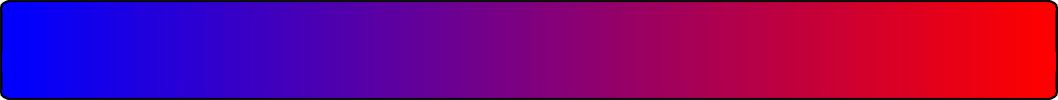
\includegraphics[width=\linewidth,height=0.05in,keepaspectratio]{../bin/colormaps/resource/pymol_blue_red_spectrum.png}};
    %
    \node(rmsdlabel) [above, inner sep=2pt] at (spectrumbarrmsd.north) {RMSD};
    %
    \node(rmsdlabelwest) [below, inner sep=6pt, align=center] at (spectrumbarrmsd.north west) {1.5 \AA};
    \node(rmsdlabeleast) [below, inner sep=6pt, align=center] at (spectrumbarrmsd.north east) {18 \AA};
    %
    \path (overlay_rmsd.north east)++(-0.25,-0.25) coordinate (arcstart);
    %
    \path[-] (dimer_roi_left.north) edge (closeup_143_rect.north west);
    \path[-] (dimer_roi_center.south) edge (closeup_310_rect.north east);
    \draw[<-, line width=0.2mm] (arcstart) arc (30:90:1);
    \node(arclabel) [below, inner sep=3pt] at (arcstart) {\ang{20}};
\end{emptypanel}
\end{fullpanelvar}
\caption[The intra-dimer interface of cardiac calsequestrin]{\textbf{\headingsubsubsectionfour}.\figurepanelcaptiona Dimer with ytterbium (Yb) sites (magenta spheres) within its interior cavity. Closeups focus on Yb positions that bridge dimer chains A and B: relatively strong coordination interactions are observed in a narrow intra-dimer cleft (right detail panel), while a site of weaker interaction and weaker occupancy is identified in the intra-dimer cavity (lower detail panel). \figurepanelcaptionb Comparison of a previously published cardiac calsequestrin dimer (1SJI) to the  more tightly-packed dimer that we report. The tightly-packed dimer results primarily from rigid body rotation of the dimer chains inward (for a single chain, we observe \ang{20} counter-clockwise rotation in the plane of the page when the other chain is fixed to the reference dimer). The inward rotation produces an increase in buried surface area (BSA) in thioredoxin domains II and III.}
\label{fig:intra_dimer_interface}
\end{figure}

\newgeometry{left=0.5cm,right=0.5cm,top=0.5cm,bottom=0.5cm}
\begin{figure}
\centering
\figuretitle{Figure~\ref{fig:inter_dimer_interface}}
\begin{fullpanelvar}
    \begin{emptypanel}{}
        %
        %
        % Overview Yb with cutaway
        % at (current page.north)
        \node(overview)[inner sep=0pt] at (current page.north) {\includegraphics[width=\linewidth,height=2.75in,keepaspectratio]{../results/inter_dimer_interface/output/tetramer_interface_overview_yb_cropped.png}};
        %
        \path (overview.north)++(-0.4,-3.5) coordinate (ybD144SW);
        \path (overview.north)++(0.4,-3) coordinate (ybD144NE);
        \node(ybD144) [fit={(ybD144SW) (ybD144NE)}, dashedrectanglefit] {};
        %
        \path (overview.north)++(-0.4,-2.4) coordinate (ybE184SW);
        \path (overview.north)++(0.4,-1.9) coordinate (ybE184NE);
        \node(ybE184) [fit={(ybE184SW) (ybE184NE)}, dashedrectanglefit] {};
        %
        \path (overview.north)++(-0.4,-4.6) coordinate (ybD348SW);            
        \path (overview.north)++(0.4,-4.1) coordinate (ybD348NE);
        \node(ybD348) [fit={(ybD348SW) (ybD348NE)}, dashedrectanglefit] {};    
        %
        \path (overview.south)++(-0.5,1.25) coordinate (ybD351SW);            
        \path (overview.south)++(0.5,1.75) coordinate (ybD351NE);
        \node(ybD351) [fit={(ybD351SW) (ybD351NE)}, dashedrectanglefit] {};
        %
        %
        \node(solventcavitylabel) [above, inner sep=5pt, align=center] at (overview.north) {Inter-Dimer\\Solvent Cavity};

        \path (overview.west)++(0.25,1) coordinate (chainA);            
        \path (overview.north)++(-2.75,-0.5) coordinate (chainB);
        \path (overview.north)++(2.75,-0.5) coordinate (chainAprime);
        \path (overview.east)++(-0.25,1) coordinate (chainBprime);

        \node(chainAlabel) [above, inner sep=2pt, align=center] at (chainA) {Chain A};
        \node(chainBlabel) [above, inner sep=2pt, align=center] at (chainB) {Chain B};
        \node(chainAprimelabel) [above, inner sep=2pt, align=center] at (chainAprime) {Chain A'};
        \node(chainBprimelabel) [above, inner sep=2pt, align=center] at (chainBprime) {Chain B'};
        %
        %
        %
        \node(D348D350)[inner sep=0pt,below=0.5cm of overview]{\includegraphics[width=\linewidth,height=1.5in,keepaspectratio]{../results/inter_dimer_interface/output/tetramer_interface_D348_D350_closeup_yb_cropped.png}};
        %
        \node(closeuprectD348D350) [fit=(D348D350), dashedrectanglefit] {};
        % Label
        \node(D348D350label) [above, inner sep=5pt, align=center] at (D348D350.north) {D348/D350 Inter-Dimer Region};
        %
        \node(D348D350Rotator) at ([yshift=0.35cm]D348D350label.north) {\AxisRotator};
        \draw[line width=0.1ex] (D348D350Rotator.west) -- (D348D350Rotator.east);
        \node(D348D350RotatorLabel)[inner sep=4pt,right] at (D348D350Rotator.east) {\ang{90}};  
        % D348_B'
        \path (D348D350.north)++(1.75,-1) coordinate (cD348chainD);
        \node(D348) [above, inner sep=0pt, font=\small, font=\bfseries] at (cD348chainD) {D348};
        % D348_A
        \path (D348D350.south)++(-2,+0.75) coordinate (cD348chainA);
        \node(D348chainA) [above, inner sep=0pt, font=\small, font=\bfseries] at (cD348chainA) {D348};
        %
        % D350_B'
        \path (D348D350.south)++(2,+0.75) coordinate (cD350chainD);
        \node(D350) [above, inner sep=0pt, font=\small, font=\bfseries] at (cD350chainD) {D350};
        % D350_A
        \path (D348D350.north)++(-2,-1) coordinate (cD350chainA);
        \node(D350chainA) [above, inner sep=0pt, font=\small, font=\bfseries] at (cD350chainA) {D350};
        %
        %
        %
        %        \path (overview.west)++(-3,-0.25) coordinate (anchor_D144E174);  %
        \node(D144E174)[inner sep=0pt,left=3.5cm of D348D350.south]{\includegraphics[width=\linewidth,height=1.75in,keepaspectratio]{../results/inter_dimer_interface/output/tetramer_interface_D144_E174_closeup_yb_cropped.png}};
        %
        \node(captionA)[inner sep=10pt,below right] at ([shift={(0cm,9cm)}]D144E174.north west) {\normalsize\textbf{\figurepanela}};
        % rect
        \node(closeuprectD144E174) [fit=(D144E174), dashedrectanglefit] {};
        % label        
        \node(D144E174label) [above, inner sep=5pt, align=center] at (D144E174.north) {D144/E174 Inter-Dimer Region};
        %
        \node(D144E174Rotator) at ([yshift=0.35cm]D144E174label.north) {\AxisRotator};
        \draw[line width=0.1ex] (D144E174Rotator.west) -- (D144E174Rotator.east);
        \node(D144E174RotatorLabel)[inner sep=4pt,right] at (D144E174Rotator.east) {\ang{90}};  
        % E184 
        \path (D144E174.west)++(0.5,1)  coordinate (cD144_B);
        \path (D144E174.east)++(-0.5,-1)  coordinate (cD144_Aprime);
        \node(D144_B) [above, inner sep=0pt, font=\small, font=\bfseries] at (cD144_B) {D144};
        \node(D144_Aprime) [above, inner sep=0pt, font=\small, font=\bfseries] at (cD144_Aprime) {D144};
        % E187 
        \path (D144E174.south west)++(0.25,0.25) coordinate (cE174_B);
        \path (D144E174.north east)++(-0.25,-0.25) coordinate (cE174_Aprime);
        \node(E174_B) [above right, inner sep=0pt, font=\small, font=\bfseries] at (cE174_B) {E174};   
        \node(E174_Aprime) [below left, inner sep=0pt, font=\small, font=\bfseries] at (cE174_Aprime) {E174};   
        %
        %
        %
        \node(D351E357)[inner sep=0pt,below=3cm of D348D350.south,anchor=center]{\includegraphics[width=\linewidth,height=1.5in,keepaspectratio]{../results/inter_dimer_interface/output/tetramer_interface_D351_E357_closeup_yb_cropped.png}};
        %
        \node(closeuprectD351E357) [fit=(D351E357), dashedrectanglefit] {};
        % Label
        \node(D351E357label) [above, inner sep=5pt, align=center] at (D351E357.north) {D351/E357 Inter-Dimer Region};
        % D351
        \path (D351E357.north)++(0,-1) coordinate (cD351);
        \node(D351) [above, inner sep=0pt, font=\small, font=\bfseries] at (cD351) {D351};
        % E357
        \path (D351E357.south)++(0,+1) coordinate (cE357);
        \node(E357) [above, inner sep=0pt, font=\small, font=\bfseries] at (cE357) {E357};
        %
        \path (closeuprectD351E357.north east)++(0,5) coordinate (ybD351_waypoint);
        \path[-] (ybD348.north west) edge (closeuprectD348D350.north west);
        \path[-] (ybD351.north east) edge (ybD351_waypoint);
        \path[-] (ybD351_waypoint) edge (closeuprectD351E357.north east);
        %
        %
        \node(E184E187)[inner sep=0pt,right=3.5cm of D351E357.north]{\includegraphics[width=\linewidth,height=3.25in,keepaspectratio]{../results/inter_dimer_interface/output/tetramer_interface_E184_E187_closeup_yb_cropped.png}};
        % rect
        \node(closeuprectE184E187) [fit=(E184E187), dashedrectanglefit] {};
        % label        
        \node(E184E187label) [above, inner sep=5pt, align=center] at (E184E187.north) {D50/K180/E184/E187 Inter-Dimer Region};
        % rotator
        % \node(E184E187Rotator) at (E184E187label.north) {\AxisRotator[rotate=90]};
        \node(E184E187Rotator) at ([yshift=0.35cm]E184E187label.north) {\AxisRotator};
        \draw[line width=0.1ex] (E184E187Rotator.west) -- (E184E187Rotator.east);
        \node(E184E187RotatorLabel)[inner sep=4pt,right] at (E184E187Rotator.east) {\ang{90}};  
        % E184 
        \path (E184E187.west)++(1,1)  coordinate (cE184);
        \node(E184) [above, inner sep=0pt, font=\small, font=\bfseries] at (cE184) {E184};
        % E187 
        \path (E184E187.north)++(-1,-0.4) coordinate (cE187);
        \node(E187) [above, inner sep=0pt, font=\small, font=\bfseries] at (cE187) {E187};        
        % D50
        \path (E184E187.east)++(-1,1) coordinate (cD50);
        \node(D50) [above, inner sep=0pt, font=\small, font=\bfseries] at (cD50) {D50};
        % K180 
        \path (E184E187.north)++(1,-0.4) coordinate (cK180);
        \node(K180) [above, inner sep=0pt, font=\small, font=\bfseries] at (cK180) {K180};
        %
        % Other side.
        %
        % E184 
        \path (E184E187.east)++(-1,-1.4)  coordinate (cE184_low);
        \node(E184_low) [above, inner sep=0pt, font=\small, font=\bfseries] at (cE184_low) {E184};
        % E187 
        \path (E184E187.south)++(1,0.25) coordinate (cE187_low);
        \node(E187_low) [above, inner sep=0pt, font=\small, font=\bfseries] at (cE187_low) {E187};        
        % D50
        \path (E184E187.west)++(1,-1.4) coordinate (cD50_low);
        \node(D50_low) [above, inner sep=0pt, font=\small, font=\bfseries] at (cD50_low) {D50};
        % K180 
        \path (E184E187.south)++(-1.5,0.25) coordinate (cK180_low);
        \node(K180_low) [above, inner sep=0pt, font=\small, font=\bfseries] at (cK180_low) {K180};
        %
        %
        \path[-] (ybD144.north west) edge (closeuprectD144E174.north west);
        \path[-] (ybE184.north east) edge (closeuprectE184E187.north east);
        %
        \path (D144E174.west)++(-0.5,0) coordinate (D144A_E174A_plot_anchor);
        %
        \node(D144A_E174A_plot)[inner sep=0pt,below=8cm of D144E174.west,anchor=west]{\input{../results/assembly_kinetics/output/kinetics_interface_mutation_D144A_E174A_85mM_K.pgf}};
        %
        \node(closeuprectD144E174plot) [fit=(D144A_E174A_plot), dashedrectanglefit] {};
        %
        \node(captionB)[inner sep=10pt,above right] at (D144A_E174A_plot.north west) {\normalsize\textbf{\figurepanelb}};
        %
        %
        %
        \node(E184A_E187A_plot)[inner sep=0pt,right=1cm of D144A_E174A_plot]{\input{../results/assembly_kinetics/output/kinetics_interface_mutation_E184A_E187A_85mM_K.pgf}};
        %
        \node(D50A_plot)[inner sep=0pt,right=0.25cm of E184A_E187A_plot]{\input{../results/assembly_kinetics/output/kinetics_interface_mutation_D50A_85mM_K.pgf}};
        %
        \node(closeuprectE184AE187A_D50Aplot) [fit=(E184A_E187A_plot)(D50A_plot), dashedrectanglefit] {};
        \node(captionC)[inner sep=10pt,above left] at (E184A_E187A_plot.north west) {\normalsize\textbf{\figurepanelc}};
        %
        \path[-] (closeuprectE184E187.south) edge (closeuprectE184AE187A_D50Aplot.north);
        \path[-] (closeuprectD144E174.south) edge (closeuprectD144E174plot.north);
    \end{emptypanel}
\end{fullpanelvar}
\caption[The inter-dimer interface of cardiac calsequestrin]{\textbf{\headingsubsubsectionfive}. \figurepanelcaptiona Yb (magenta spheres) bound within the walled pocket formed by the inter-dimer interface, with closeups of ytterbium site at E184 and E187, D348 and D350, and D351 and D357. Thioredoxin domain II of chain A' (blue) is omitted to allow visualization of the interior of the solvent pocket formed by the inter-dimer interface. \figurepanelcaptionb Turbidity assays after alanine mutagenesis of putative calcium-binding residues D144 and E174. \figurepanelcaptionc Left: turbidity assay after alanine mutagenesis of putative calcium-binding residues E184 and E187. Right: turbidity assay after alanine mutagenesis of the D50 residue that participates in a salt bridge with K180, adjacent to the E184/E187 ligand site.}
\label{fig:inter_dimer_interface}
\end{figure}
%\end{landscape}
\restoregeometry






\newgeometry{left=0.5cm,right=0.5cm,top=0.5cm,bottom=0.5cm}
\begin{figure}[hp]
\figuretitle{Figure~\ref{fig:filament_cavity}}
\begin{fullpanelvar}
    \begin{emptypanel}{}
        %
        \node(axialdimer)[inner sep=0pt,below right]{\includegraphics[width=\linewidth,height=1.25in,keepaspectratio]{../results/cavity/output/dimer_cavity_axial_cropped.png}};
        %
        \path (axialdimer.north)++(-0.25,-1.35) coordinate (axialdimerROISW1);           
        \path (axialdimer.north)++(0.25,-2.1) coordinate (axialdimerROINE1);
        \node(axialdimerROIrect) [fit={(axialdimerROISW1) (axialdimerROINE1)}, dashedrectanglefit] {};
        %
        \node(captionA)[inner sep=0pt,above left] at (axialdimer.north west) {\normalsize\textbf{\figurepanela}};
        %
        \path (axialdimer.south west)++(0.4,-0.5) coordinate (chainArotated);           
        \path (axialdimer.south east)++(-0.4,-0.5) coordinate (chainBrotated);
        %
        \node(chainArotatedlabel) [above, inner sep=2pt, align=center] at (chainArotated) {Chain A};
        \node(chainBrotatedlabel) [above, inner sep=2pt, align=center] at (chainBrotated) {Chain B};
        %
        %
        %
        \node(axialdimerapbs)[inner sep=0pt,right=0.5cm of axialdimer]{\includegraphics[width=\linewidth,height=1.25in,keepaspectratio]{../results/cavity/output/dimer_cavity_apbs_axial_no_ramp_cropped.png}};
        %
        \node(axialdimerlabel) [below, inner sep=2pt, align=center] at (axialdimerapbs.south) {Solvent-Exposed Side\\(Filament End Cap)};
        %
        \path (axialdimerapbs.north)++(-0.25,-1.35) coordinate (axialdimerapbsROISW1);   
        \path (axialdimerapbs.north)++(0.25,-2.1) coordinate (axialdimerapbsROINE1);
        \node(axialdimerapbsROIrect) [fit={(axialdimerapbsROISW1) (axialdimerapbsROINE1)}, dashedrectanglefit] {};
        %
        \path[-] (axialdimerROIrect.east) edge (axialdimerapbsROIrect.west);
        %
        %
        %
        \node(spectrumbar)[inner sep=0pt,right=0.5cm of axialdimerapbs.east]{\rotatebox[origin=c]{-90}{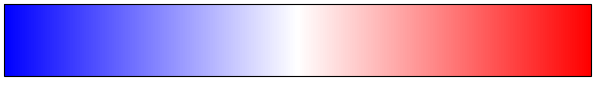
\includegraphics[width=\linewidth,height=0.15in,keepaspectratio]{../bin/colormaps/resource/matplotlib_bwr.png}}};
        %
        \node(apbslabel) [above, inner sep=6pt] at (spectrumbar.north) {30 kT/e};
        \node(apbslabel) [below, inner sep=6pt] at (spectrumbar.south) {-30 kT/e};       
        %
        %
        %
        \node(tetramer)[inner sep=0pt,right=1cm of spectrumbar.east]{\includegraphics[width=\linewidth,height=1.25in,keepaspectratio]{../results/cavity/output/tetramer_cavity_apbs_side_no_ramp_cropped.png}};
        %
        \node(captionB)[inner sep=0pt,above left] at (tetramer.north west) {\normalsize\textbf{\figurepanelb}};
        %
        \path (tetramer.north)++(-0.5,-0.95) coordinate (tetramerROISW1);            
        \path (tetramer.north)++(0.5,-1.8) coordinate (tetramerROINE1);
        \node(tetramerROIrect) [fit={(tetramerROISW1) (tetramerROINE1)}, dashedrectanglefit] {};
        %
        %
        \path (tetramer.west)++(-0.25,0.5) coordinate (chainA_tetramer);           
        \path (tetramer.north)++(-1.5,0) coordinate (chainB_tetramer);
        \path (tetramer.north)++(1.5,0) coordinate (chainAprime_tetramer);
        \path (tetramer.east)++(0.25,0.5) coordinate (chainBprime_tetramer);
        %
        \node(chainAlabel) [above, inner sep=2pt, align=center] at (chainA_tetramer) {Chain A};
        \node(chainBlabel) [above, inner sep=2pt, align=center] at (chainB_tetramer) {Chain B};
        \node(chainAprimelabel) [above, inner sep=2pt, align=center] at (chainAprime_tetramer) {Chain A'};
        \node(chainBprimelabel) [above, inner sep=2pt, align=center] at (chainBprime_tetramer) {Chain B'};
        %
        \node(D144_E174_closeup)[inner sep=0pt,right=1cm of tetramer.east,anchor=west]{\includegraphics[width=\linewidth,height=1in,keepaspectratio]{../results/cavity/output/tetramer_cavity_D144_E174_closeup_no_ramp_cropped.png}};
        %
        \node(closeuprectD144E174) [fit=(D144_E174_closeup), dashedrectanglefit] {};
        %
        \path[-] (tetramerROIrect.north east) edge (closeuprectD144E174.north west);
        %
        \path (D144_E174_closeup.south west)++(0.5,-0.65) coordinate (cE174label);
        \path (D144_E174_closeup.west)++(1.125,-0.65) coordinate (cE174);
        \node(E174) [above, inner sep=3pt] at (cE174label) {E174};
        \path[-] (E174.north) edge (cE174.south);
        %
        \path (D144_E174_closeup.south east)++(-0.5,-0.65) coordinate (cD144label);
        \path (D144_E174_closeup.east)++(-1.125,-0.3) coordinate (cD144);
        \node(D144) [above, inner sep=3pt] at (cD144label) {D144};
        \path[-] (D144.north) edge (cD144.south);
        %
        \node(filament)[inner sep=0pt,below=5.5cm of axialdimer.west,anchor=west]{\includegraphics[width=\linewidth,height=2in,keepaspectratio]{../results/cavity/output/filament_cavity_and_yb_blend_cutaway_cropped.png}};
        %
        \node(captionC)[inner sep=0pt,above left] at (filament.north west) {\normalsize\textbf{\figurepanelc}};
        %
     \end{emptypanel}
\end{fullpanelvar}
\caption[The electronegative lumen within the cardiac calsequestrin filament]{\textbf{\headingsubsectionsix}. \figurepanelcaptiona Left panel: the interior cavity of the dimer viewed down its long axis. Residues that participate in the coordination of Yb atoms within the intra-dimer cleft (Figure~\ref{fig:intra_dimer_interface}) are shown as sticks. All other residues are rendered as surface. Right panel: APBS-generated electrostatic surface of the same region. \figurepanelcaptionb The lumen is continuous down the length of filament because of the large solvent cavity formed at each dimer-dimer interface. The APBS-generated electrostatic surface of the lumen (as traced by HOLLOW using a 1.4 \AA probe) is shown, with closeup of residues D144 and E174 deep within the electronegative cavity. \figurepanelcaptionc View of the filament and its continuous interior cavity, with Yb sites shown as purple spheres.}
\label{fig:filament_cavity}
\end{figure}
\restoregeometry
\begin{figure}
\figuretitle{Figure~\ref{fig:inter_dimer_interface_cpvt}}
\begin{fullpanelvar}
    \begin{emptypanel}{}
        \node(overview1)[inner sep=0pt,below right]{\includegraphics[width=\linewidth,height=1.75in,keepaspectratio]{../results/inter_dimer_interface/output/tetramer_interface_overview_CPVT_cropped.png}};
        %
        \node(captionA)[inner sep=10pt,above left] at (overview1.north west) {\normalsize\textbf{\figurepanela}};
        %
        \path (overview1.north)++(-1,-2.5) coordinate (S173SW1);            
        \path (overview1.north)++(-0.375,-1.75) coordinate (S173NE1);
        \node(S173one) [fit={(S173SW1) (S173NE1)}, dashedrectanglefit] {};
        %
        \path (overview1.north)++(0.375,-2.5) coordinate (S173SW2);           
        \path (overview1.north)++(1,-1.75) coordinate (S173NE2);
        \node(S173two) [fit={(S173SW2) (S173NE2)}, dashedrectanglefit] {};
        %
        %
        \path (overview1.north)++(-0.5,-1.75) coordinate (K180SW1);            
        \path (overview1.north)++(0,-1.125) coordinate (K180NE1);
        \node(K180one) [fit={(K180SW1) (K180NE1)}, dashedrectanglefit] {};
        %
        \path (overview1.north)++(0,-1.75) coordinate (K180SW2);           
        \path (overview1.north)++(0.5,-1.125) coordinate (K180NE2);
        \node(K180two) [fit={(K180SW2) (K180NE2)}, dashedrectanglefit] {};
        %
        \path (overview1.west)++(0,1) coordinate (chainA);           
        \path (overview1.north)++(-2.4,-0.5) coordinate (chainB);
        \path (overview1.north)++(2.4,-0.5) coordinate (chainAprime);
        \path (overview1.east)++(-0.25,1) coordinate (chainBprime);

        \node(chainAlabel) [above, inner sep=2pt, align=center] at (chainA) {Chain A};
        \node(chainBlabel) [above, inner sep=2pt, align=center] at (chainB) {Chain B};
        \node(chainAprimelabel) [above, inner sep=2pt, align=center] at (chainAprime) {Chain A'};
        \node(chainBprimelabel) [above, inner sep=2pt, align=center] at (chainBprime) {Chain B'};
        %
        %
        %
        \node(closeup180)[inner sep=0pt,right=1.5cm of overview1]{\includegraphics[width=\linewidth,height=1.5in,keepaspectratio]{../results/inter_dimer_interface/output/tetramer_interface_K180_closeup_yb_cropped.png}};
        \node(closeup180rect) [fit=(closeup180), dashedrectanglefit] {};
        %
        \node(K180_ROI_label) [above, inner sep=5pt, align=center] at (closeup180.north) {D50/K180/E184/E187 Inter-Dimer Region};
        %
        \node(K180Rotator) at ([yshift=0.35cm]K180_ROI_label.north) {\AxisRotator};
        \draw[line width=0.1ex] (K180Rotator.west) -- (K180Rotator.east);
        \node(K180RotatorLabel)[inner sep=4pt,right] at (K180Rotator.east) {\ang{60}};  
        %
        \node(captionB)[inner sep=10pt,above left] at (closeup180.north west) {\normalsize\textbf{\figurepanelb}};
        %
        % E184 
        \path (closeup180.east)++(-1,-1.4)  coordinate (cE184);
        \node(E184_label) [above, inner sep=0pt, font=\small, font=\bfseries] at (cE184) {E184};
        % E187 
        \path (closeup180.east)++(-0.4,0.4) coordinate (cE187);
        \node(E187_label) [above, inner sep=0pt, font=\small, font=\bfseries] at (cE187) {E187};
        % D50
        \path (closeup180.west)++(0.75,0.4) coordinate (cD50);
        \node(D50_label) [above, inner sep=0pt, font=\small, font=\bfseries] at (cD50) {D50};
        % K180 
        \path (closeup180.west)++(2.2,0.3) coordinate (cK180);
        \node(K180) [above, inner sep=0pt, font=\small, font=\bfseries] at (cK180) {K180};
        %
        \path[-] (K180two.north east) edge (closeup180rect.north west);
        %
        %
        %
        \node(closeup173)[inner sep=0pt,below=3.5cm of overview1.south west,anchor=west]{\includegraphics[width=\linewidth,height=1.5in,keepaspectratio]{../results/inter_dimer_interface/output/tetramer_interface_S173_closeup_cropped.png}};
        \node(closeup173rect) [fit=(closeup173), dashedrectanglefit] {};
        %
        \node(captionC)[inner sep=10pt,above left] at (closeup173.north west) {\normalsize\textbf{\figurepanelc}};
        %
        \node(S173_ROI_label) [above, inner sep=5pt, align=center] at (closeup173.north) {K87/S173/D325 Inter-Dimer Region};
        % S173
        \path (closeup173.west)++(1.5,0.25) coordinate (cS173);
        \node(S173) [above, inner sep=0pt, font=\small, font=\bfseries] at (cS173) {S173};
        % D325
        \path (closeup173.south)++(-1.25,+0.25) coordinate (cD325);
        \node(D325) [above, inner sep=0pt, font=\small, font=\bfseries] at (cD325) {D325}; 
        % D319
        \path (closeup173.south)++(2,1) coordinate (cD319);
        \node(D319) [above, inner sep=0pt, font=\small, font=\bfseries] at (cD319) {D319}; 
        % K87
        \path (closeup173.east)++(-1.25,0.5) coordinate (cK87);
        \node(K87) [above, inner sep=0pt, font=\small, font=\bfseries] at (cK87) {K87}; 
        %
        \path[-] (S173one.south west) edge (closeup173rect.north west);
        %
        %
        %
        \node(D325A_plot)[inner sep=0pt,right=1.5cm of closeup173.east,anchor=west]{\input{../results/assembly_kinetics/output/kinetics_interface_mutation_D325A_85mM_K.pgf}};
        %
        \node(captionD)[inner sep=10pt,above left] at (D325A_plot.north west) {\normalsize\textbf{\figurepaneld}};
        %
        \node(closeuprectD325Aplot) [fit=(D325A_plot), dashedrectanglefit] {};
        %
        \path[-] (closeup173rect.east) edge (closeuprectD325Aplot.west);
    \end{emptypanel}
\end{fullpanelvar}
\caption[The S173 residue is at the cardiac calsequestrin inter-dimer interface]{\textbf{\headingsubsectionseven}. \figurepanelcaptiona The S173 residue, site of the newly-identified S173I putative disease mutation, is located at a highly hydrophilic 3-protomer interface within the inter-dimer contact region. Disruption of this hydrophilic pocket by hydrophobic substitution leads to filamentation defect. The inter-dimer interface is shown with interface residues in the S173 region rendered as spheres. the closeup panel shows a charged pocket at the location of the CPVT-associated S173I mutation is found. In this pocket, 3 different thioredoxin domains from 3 distinct chains interact (K87, S173, D325). \figurepanelcaptionb Turbidity assay with the D325A mutation.}
\label{fig:inter_dimer_interface_cpvt}
\end{figure}
\newgeometry{left=0.5cm,right=0.5cm,top=0.5cm,bottom=0.5cm}
\begin{figure}
\centering
\figuretitle{Figure~\ref{fig:graphical_summary}}
    % All about specifying coords: https://stuff.mit.edu/afs/athena/contrib/tex-contrib/beamer/pgf-1.01/doc/generic/pgf/version-for-tex4ht/en/pgfmanualse8.html
    \tikzset{
        monomerA/.pic = {
            \draw[fill=orange,rounded corners] (-0.5,0)  
            -- ++(0.75,0) 
            -- ++(0.5,-1) 
            -- ++(-1.25,0) 
            -- cycle;
        }
    }
    \tikzset{
        monomerAmutantIntra/.pic = {
            \draw[fill=red,rounded corners] (-0.5,0) node(monomerAanchor)[inner sep=14] {}
            -- ++(0.75,0) 
            -- ++(0.5,-1) 
            -- ++(-1.25,0) 
            -- cycle;
            \draw[fill=LimeGreen,rounded corners] (-0.5,0) node(monomerAanchor2)[inner sep=14] {} 
            -- ++(0.625,0) 
            -- ++(0.5,-1) 
            -- ++(-1.125,0) 
            -- cycle;
            % Was previously using a start to indicate the mutant.
            % \node[star,star points=5, draw, fill=red,star point ratio=2.25,inner sep=0pt,minimum height=0.5cm] at ([xshift=-0.05cm]monomerAanchor.south east) {};
        }
    }
    \tikzset{
        monomerAmutantInter/.pic = {
            \draw[fill=red,rounded corners] (-0.5,0) node(monomerAanchor)[inner sep=14] {}
            -- ++(0.75,0) 
            -- ++(0.5,-1) 
            -- ++(-1.25,0) 
            -- cycle;
            \draw[fill=LimeGreen,rounded corners] (-0.375,0) node(monomerAanchor2)[inner sep=14] {} 
            -- ++(0.625,0) 
            -- ++(0.5,-1) 
            -- ++(-1.125,0) 
            -- cycle;
        }
    }
    % "B" chain
    \tikzset{
        monomerB/.pic = {
            \draw[fill=orange,rounded corners] (-0.5,0)  
            -- ++(1.25,0) 
            -- ++(0,-1) 
            -- ++(-0.75,0) 
            -- cycle;
        }
    }
    \tikzset{
        monomerBmutantIntra/.pic = {
            \draw[fill=red,rounded corners] (-0.5,0) node(monomerBanchor)[inner sep=14] {}
            -- ++(1.25,0) 
            -- ++(0,-1) 
            -- ++(-0.75,0) 
            -- cycle;
            \draw[fill=LimeGreen,rounded corners] (-0.375,0) node(monomerBanchor)[inner sep=14] {} 
            -- ++(1.125,0) 
            -- ++(0,-1) 
            -- ++(-0.625,0) 
            -- cycle;
        }
    }
    \tikzset{
        monomerBmutantInter/.pic = {
            \draw[fill=red,rounded corners] (-0.5,0) node(monomerBanchor)[inner sep=14] {}
            -- ++(1.25,0) 
            -- ++(0,-1) 
            -- ++(-0.75,0) 
            -- cycle;
            \draw[fill=LimeGreen,rounded corners] (-0.5,0) node(monomerBanchor)[inner sep=14] {} 
            -- ++(1.125,0) 
            -- ++(0,-1) 
            -- ++(-0.625,0) 
            -- cycle;
        }
    }
    \begin{emptypanel}{}
        % https://tex.stackexchange.com/questions/185279/anchoring-tikz-pics
        %
        \node(legendTitle)[align=center,font=\small,font=\bfseries, minimum size=2cm] at (current page.north) {Heterozygous Missense Genotypes};
        \node(legendCenter)[align=center,below=0.125cm of legendTitle.south] {};
        %
%        \pic at ([xshift=-0.45cm,yshift=-0.6cm]legendWT.north) {monomerA};
%        \pic at ([xshift=0.45cm,yshift=-0.6cm]legendWT.north) {monomerB};
        %
        \node(legendIntra)[left=1cm of legendCenter.west,align=center] {\textit{Intra}-Dimer Mutant};
        %
        \pic at ([xshift=-1cm,yshift=-0.6cm]legendIntra.north) {monomerA};
        \node(X1)[align=center,color=red,font=\bfseries, font=\large, minimum size=2cm] at ([xshift=0cm,yshift=-0.7cm]legendIntra.south) {\Large \bf X};
        \pic at ([xshift=0.75cm,yshift=-0.6cm]legendIntra.north) {monomerBmutantIntra};
        %
        \node(legendInter)[right=1cm of legendCenter.east,align=center] {\textit{Inter}-Dimer Mutant};
        %
        \pic at ([xshift=-0.45cm,yshift=-0.6cm]legendInter.north) {monomerA};
        \pic at ([xshift=0.45cm,yshift=-0.6cm]legendInter.north) {monomerBmutantInter};
        %
        \draw[thick] ($(legendIntra.north west)+(-1,0.5)$) rectangle ($(legendInter.south east)+(1,-1.75)$);
    \end{emptypanel}
    \vspace{0.75cm}
    \begin{emptypanel}{}
        \node(genotypesLabel)[below right,align=center,font=\small,font=\bfseries, minimum size=2cm] {Genotype\\and\\Interface};
        %
%        \node(chainTypesLabel)[right=2cm of genotypesLabel.east,align=center,font=\small,font=\bfseries, minimum size=2cm] {Protomers};
        %
        \node(retainedLabel)[right=2.5cm of genotypesLabel.east,align=center,font=\small,font=\bfseries, minimum size=2cm] {Retained\\and\\Functional};
        % 
        \node(traffickedLabel)[right=2cm of retainedLabel.east,align=center,font=\small,font=\bfseries, minimum size=2cm] {Non-Filamented,\\Exported};
        %
        % First separator
        %
        \path (genotypesLabel.south)++(-2,-0.5) coordinate (Separator1Left);
        \path (traffickedLabel.south)++(2,-0.5) coordinate (Separator1Right);
        \path[-] (Separator1Left) edge (Separator1Right);
        %
        %
        \node(hetIntraLabel)[below=1cm of genotypesLabel.south,align=center,font=\small] {Heterozygous\\\textit{Intra}-Dimer Mutant};
        %
        % \node(IntraChainTypes)[below=1cm of chainTypesLabel.south,align=center] {};
        % %
        % \pic at ([xshift=-0.75cm]IntraChainTypes.north) {monomerA};
        % \pic at ([xshift=0.75cm]IntraChainTypes.south) {monomerBmutantIntra};
        %
        \node(hetIntraHomoWT)[below=1cm of retainedLabel.south,align=center] {};
        %
        \pic at ([xshift=-0.45cm]hetIntraHomoWT.north) {monomerA};
        \pic at ([xshift=0.45cm]hetIntraHomoWT.north) {monomerB};
        \node(retainedPctIntra)[below=1cm of hetIntraHomoWT.south,align=center,font=\bfseries] {\SI{50}{\percent}};
        %
        \node(hetIntraHomoMut)[below=1cm of traffickedLabel.south,align=center] {};
        %
        \pic at ([xshift=-1cm]hetIntraHomoMut.north) {monomerAmutantIntra};
        \node(X2)[align=center,color=red,font=\large,font=\bfseries, minimum size=2cm] at ([xshift=0cm,yshift=-0.3cm]hetIntraHomoMut.south) {\Large \bf X};
        \pic at ([xshift=0.75cm]hetIntraHomoMut.north) {monomerBmutantIntra};
        %
        %
        %
        \path (genotypesLabel.south)++(-2,-3) coordinate (separator2Left);
        \path (traffickedLabel.south)++(2,-3) coordinate (separator2Right);
        \path[-] (separator2Left) edge (separator2Right);
        %
        %
        %
        \node(hetInterLabel)[below=3.5cm of genotypesLabel.south,align=center,font=\small] {Heterozygous\\\textit{Inter}-Dimer Mutant};
        %
        % \node(hetInterChainTypes)[below=3.5cm of chainTypesLabel.south,align=center] {};
        % %
        % \pic at ([xshift=-0.75cm]hetInterChainTypes.north) {monomerA};
        % \pic at ([xshift=0.75cm]hetInterChainTypes.south) {monomerBmutantInter};
        %
        % Retained
        %
        \node(hetInterHomoWT)[below=3.5cm of retainedLabel.south,align=center] {};
        %
        \pic at ([xshift=-0.45cm]hetInterHomoWT.north) {monomerA};
        \pic at ([xshift=0.45cm]hetInterHomoWT.north) {monomerB};
        \node(retainedPctInter)[below=1cm of hetInterHomoWT.south,align=center,font=\bfseries] {\SI{25}{\percent}};
        %
        % Exported
        %
        \node(hetInterHet1)[below=3.5cm of traffickedLabel.south,align=center] {};
        %
        \pic at ([xshift=-0.45cm]hetInterHet1.north) {monomerA};
        \pic at ([xshift=0.45cm]hetInterHet1.north) {monomerBmutantInter};

        \node(hetInterHet2)[below=1.25cm of hetInterHet1.south,align=center] {};

        \pic at ([xshift=-0.45cm]hetInterHet2.north) {monomerAmutantInter};
        \pic at ([xshift=0.45cm]hetInterHet2.north) {monomerB};

        \node(hetInterHomoMut)[below=1.25cm of hetInterHet2.south,align=center] {};

        \pic at ([xshift=-0.45cm]hetInterHomoMut.north) {monomerAmutantInter};
        \pic at ([xshift=0.45cm]hetInterHomoMut.north) {monomerBmutantInter};
    \end{emptypanel}
    \vspace{0.75cm}
\caption[Disease inheritance patterns differ by location of mutation]{\textbf{Heterozygously-carried mutations at different calsequestrin interfaces have different disease inheritance patterns.} Mutations that inhibit dimerization are likely to cause penetrant disease only when carried recessively - a consequence of export of mutant monomers from the ER/SR. However, mutations that inhibit dimer-dimer interaction are likely to have dominant effect - a consequence of the fact that only \SI{25}{\percent} of dimers are functional for the purpose of filamentation.}
\label{fig:graphical_summary}
\end{figure}
\restoregeometry
\clearpage
% \subsection{Supplemental Figures}
% Optionally make clicky links to the online file using \verb!\href{url}{description}!.
% Reset the figure counter and add "S" to the figure caption (e.g. "Figure S1"). 
\setcounter{figure}{0}
\setcounter{table}{0}
\renewcommand{\thefigure}{S\arabic{figure}}
\renewcommand{\thetable}{S\arabic{table}}
\begin{figure}[!ht]
\centering
\figuretitle{Figure~\ref{fig:biochemistry_supplement}}
\hfill
\begin{fullpanelvar}
    \begin{emptypanel}{}
        \node(WT_EDTA_plot)[inner sep=0pt,above right]{\input{../results/assembly_kinetics/output/kinetics_WT_EDTA.pgf}};
        %
        \node(captionA)[inner sep=0pt,above left] at (WT_EDTA_plot.north west) {\normalsize\textbf{\figurepanela}};
        %
        \node(S173I_No_K_plot)[inner sep=0pt,right=2cm of WT_EDTA_plot.east, anchor=west]{\input{../results/assembly_kinetics/output/kinetics_CPVT_mutation_S173I_0mM_K.pgf}};
        %
        \node(captionB)[inner sep=0pt,above left] at (S173I_No_K_plot.north west) {\normalsize\textbf{\figurepanelb}};
        %
    \end{emptypanel}
\end{fullpanelvar}        
\hfill
\rowspacer
\caption[Multimerization kinetics of the S173I mutant observed in 0 mM KCl]{\textbf{Opacification of calsequestrin samples in the presence of calcium is reversible upon chelation. Multimerization Kinetics of the S173I Mutant Observed in 0 mM KCl show that S173I mutant is functional. Related to Figure~\ref{fig:S173I_genetics_and_biochemistry}.} \figurepanelcaptiona Turbidity assay with stoichiometric addition of EDTA demonstrates immediate reversal of opacification. \figurepanelcaptionb Turbidity assay for the S173I mutant.}
\label{fig:biochemistry_supplement}
\end{figure}
\newgeometry{left=0.5cm,right=0.5cm,top=0.5cm,bottom=0.5cm}
\thispagestyle{empty}
\begin{landscape}
\begin{figure}[!ht]
\centering
\newcommand{\tetramerheight}{1.25in}
\figuretitle{Figure~\ref{fig:inter_dimer_interface_BSA_comparison}}
\begin{fullpanelvar}
    \begin{emptypanel}{}
        \node(deo_native)[inner sep=0pt, below right] {\includegraphics[width=\linewidth,height=\tetramerheight,keepaspectratio]{../results/inter_dimer_comparison/output/tetramer_deo_native_oriented_cropped.png}};
        %
        \node (deo_native_table) [inner sep=10pt,anchor=north] at (deo_native.south) {
            \begin{tabular}{c c}
                Interface Chains & BSA (\AA\textsuperscript{2}) \\
                \hline
                \input{../results/inter_dimer_comparison/output/table_interface_comparison_tetramer_deo_native.tex}
                % B, A’ & 734.0 \\
                % A, A’ & 382.0 \\
                % B, B’ & 381.0 \\
                % A, B’ & 101.0
            \end{tabular}
        };
        %
        \node(6OVW_label) [above, inner sep=3pt, align=center] at (deo_native.north) {6OVW (This Study)\\Similar: 6OWW};
        %
        \node(1a8y)[inner sep=0pt,right=1cm of deo_native] {\includegraphics[width=\linewidth,height=\tetramerheight,keepaspectratio]{../results/inter_dimer_comparison/output/tetramer_1a8y_oriented_cropped.png}};
        %
        \node(1a8y_label) [above, inner sep=3pt, align=center] at (1a8y.north) {1A8Y\\Similar: 3TRP, 3TRQ, 3US3, 3V1W, 5CRD, 5KN0, 5KN3};
        %
        \node (1a8y_table) [inner sep=10pt,anchor=north] at (1a8y.south) {
            \begin{tabular}{c c}
                Interface Chains & BSA (\AA\textsuperscript{2}) \\
                \hline
                \input{../results/inter_dimer_comparison/output/table_interface_comparison_tetramer_1a8y.tex}
            \end{tabular}
        };
        %
        \node(1sji)[inner sep=0pt,right=1cm of 1a8y] {\includegraphics[width=\linewidth,height=\tetramerheight,keepaspectratio]{../results/inter_dimer_comparison/output/tetramer_1sji_oriented_cropped.png}};
        %
        \node(1sji_label) [above, inner sep=3pt, align=center] at (1sji.north) {1SJI};
        %
        \node (1sji_table) [inner sep=10pt,anchor=north] at (1sji.south) {
            \begin{tabular}{c c}
                Interface Chains & BSA (\AA\textsuperscript{2}) \\
                \hline
                \input{../results/inter_dimer_comparison/output/table_interface_comparison_tetramer_1sji.tex}
            \end{tabular}
        };
        %
        \node(2vaf)[inner sep=0pt,right=1cm of 1sji] {\includegraphics[width=\linewidth,height=\tetramerheight,keepaspectratio]{../results/inter_dimer_comparison/output/tetramer_2vaf_oriented_cropped.png}};
        %
        \node(2vaf_label) [above, inner sep=3pt, align=center] at (2vaf.north) {2VAF};
        %
        \node (2vaf_table) [inner sep=10pt,anchor=north] at (2vaf.south) {
            \begin{tabular}{c c}
                Interface Chains & BSA (\AA\textsuperscript{2}) \\
                \hline
                \input{../results/inter_dimer_comparison/output/table_interface_comparison_tetramer_2vaf.tex}
            \end{tabular}
        };
        %
        \node(3uom)[inner sep=0pt,below=7cm of deo_native.west,anchor=west] {\includegraphics[width=\linewidth,height=\tetramerheight,keepaspectratio]{../results/inter_dimer_comparison/output/tetramer_3uom_oriented_cropped.png}};
        %
        \node(3uom_label) [above, inner sep=3pt, align=center] at (3uom.north) {3UOM};
        %
        \node (3uom_table) [inner sep=10pt,anchor=north] at (3uom.south) {
            \begin{tabular}{c c}
                Interface Chains & BSA (\AA\textsuperscript{2}) \\
                \hline
                \input{../results/inter_dimer_comparison/output/table_interface_comparison_tetramer_3uom.tex}
            \end{tabular}
        };
        %
        \node(5cre)[inner sep=0pt,right=1cm of 3uom] {\includegraphics[width=\linewidth,height=\tetramerheight,keepaspectratio]{../results/inter_dimer_comparison/output/tetramer_5cre_oriented_cropped.png}};
        %
        \node(5cre_label) [above, inner sep=3pt, align=center] at (5cre.north) {5CRE};
        %
        \node (5cre_table) [inner sep=10pt,anchor=north] at (5cre.south) {
            \begin{tabular}{c c}
                Interface Chains & BSA (\AA\textsuperscript{2}) \\
                \hline
                \input{../results/inter_dimer_comparison/output/table_interface_comparison_tetramer_5cre.tex}
            \end{tabular}
        };
        %
        \node(5crg)[inner sep=0pt,right=1cm of 5cre] {\includegraphics[width=\linewidth,height=\tetramerheight,keepaspectratio]{../results/inter_dimer_comparison/output/tetramer_5crg_oriented_cropped.png}};
        %
        \node(5crg_label) [above, inner sep=3pt, align=center] at (5crg.north) {5CRG\\Similar: 5CRH};
        %
        \node (5crg_table) [inner sep=10pt,anchor=north] at (5crg.south) {
            \begin{tabular}{c c}
                Interface Chains & BSA (\AA\textsuperscript{2}) \\
                \hline
                \input{../results/inter_dimer_comparison/output/table_interface_comparison_tetramer_5crg.tex}
            \end{tabular}
        };
        %
        \node(5kn1)[inner sep=0pt,right=1cm of 5crg] {\includegraphics[width=\linewidth,height=\tetramerheight,keepaspectratio]{../results/inter_dimer_comparison/output/tetramer_5kn1_oriented_cropped.png}};
        %
        \node(5kn1_label) [above, inner sep=3pt, align=center] at (5kn1.north) {5KN1\\Similar: 5KN2};
        %
        \node (5kn1_table) [inner sep=10pt,anchor=north] at (5kn1.south) {
            \begin{tabular}{c c}
                Interface Chains & BSA (\AA\textsuperscript{2}) \\
                \hline
                \input{../results/inter_dimer_comparison/output/table_interface_comparison_tetramer_5kn1.tex}
            \end{tabular}
        };
        %
    \end{emptypanel}
\end{fullpanelvar}    
\caption[Comparison of buried surface area (BSA) at putative dimer-dimer multimerization interfaces observed in all published calsequestrin structures]{\textbf{The Dimer-to-Dimer Interface of the New Candidate Cardiac Calsequestrin Filament Is Characterized by All-by-All Contacts and Greater Buried Surface Area (BSA) Compared to All Other Published Calsequestrin Structures, Related to Figure~\ref{fig:filament_overview}.} For each published calsequestrin structure, the dimer-to-dimer interface with the greatest buried surface area is shown. Residues with buried surface area at the interface are rendered as spheres. Orange, chain A; forest, chain B; sky blue, chain A'; yellow, chain B'. Where similar PDB codes are listed, dimer-to-dimer interfaces are roughly are isomorphous with the example structure shown, although the space group and unit cell used to determine the structure sometimes differ.} 
\label{fig:inter_dimer_interface_BSA_comparison}
\end{figure}
\end{landscape}
\restoregeometry

\begin{figure}[!ht]
\centering
\figuretitle{Figure~\ref{fig:intra_dimer_interface_maps}}
\begin{fullpanelvar}
    \begin{emptypanel}{\figurepanela}
        %
        \node(E143nativemap)[inner sep=0pt,below right]{\includegraphics[width=1.75in,keepaspectratio]{../results/dimer_interface/output/dimer_interface_E143_closeup_native_map_cropped.png}};
        %
        \node(belowcaption)[below, inner sep=5pt] at (E143nativemap.south) {Native map at 1.5 $\sigma$};
        %
        \node(E143ybmap)[inner sep=0pt,right=1cm of E143nativemap]{\includegraphics[width=1.75in,keepaspectratio]{../results/dimer_interface/output/dimer_interface_E143_closeup_yb_map_cropped.png}};
        %
        \node(belowcaption)[below, inner sep=5pt] at (E143ybmap.south) {Yb-complexed map at 1.5 $\sigma$};
        %
        \node(E143anommap)[inner sep=0pt,right=0cm and 1cm of E143ybmap]{\includegraphics[width=1.75in,keepaspectratio]{../results/dimer_interface/output/dimer_interface_E143_closeup_yb_map_anom_cropped.png}};
        %
        \node(belowcaption)[below, inner sep=5pt] at (E143anommap.south) {Yb-complexed anomalous map at 3.0 $\sigma$};
    \end{emptypanel}
\end{fullpanelvar}
\rowspacersmall
\begin{fullpanelvar}
    \begin{emptypanel}{\figurepanelb}
        %
        \node(D310nativemap)[inner sep=0pt,below right]{\includegraphics[width=1.75in,keepaspectratio]{../results/dimer_interface/output/dimer_interface_D310_closeup_native_map_cropped.png}};
        %
        \node(belowcaption)[below, inner sep=5pt] at (D310nativemap.south) {Native map at 1.5 $\sigma$};
        %
        \node(D310ybmap)[inner sep=0pt,right=1cm of D310nativemap]{\includegraphics[width=1.75in,keepaspectratio]{../results/dimer_interface/output/dimer_interface_D310_closeup_yb_map_cropped.png}};
        %
        \node(belowcaption)[below, inner sep=5pt] at (D310ybmap.south) {Yb-complexed map at 1.5 $\sigma$};
        %
        \node(D310anommap)[inner sep=0pt,right=1cm of D310ybmap]{\includegraphics[width=1.75in,keepaspectratio]{../results/dimer_interface/output/dimer_interface_D310_closeup_yb_map_anom_cropped.png}};
        %
        \node(belowcaption)[below, inner sep=5pt] at (D310anommap.south) {Yb-complexed anomalous map at 3.0 $\sigma$};
    \end{emptypanel}
\end{fullpanelvar}
\caption[Maps for Yb-Binding Sites at the Cardiac Calsequestrin Intra-Dimer Interface]{\textbf{Electron Density and Anomalous Difference Maps for Yb-Binding Sites at the Cardiac Calsequestrin Intra-Dimer Interface, Related to Figure~\ref{fig:intra_dimer_interface}.} \figurepanelcaptiona Electron density and anomalous difference Maps for the D140/E143/E147 region of interest. \figurepanelcaptionb Electron density and anomalous difference maps for the D310 region of interest.}
\label{fig:intra_dimer_interface_maps}
\end{figure}





\begin{figure}[!ht]
\centering
\figuretitle{Figure~\ref{fig:intra_dimer_interface_6OVW_vs_other_overlay}}
\begin{fullpanelvar}
    \begin{emptypanel}{}
        %
        % 2VAF
        \node(pdb_2vaf)[inner sep=0pt,below right]{\includegraphics[height=0.75in,keepaspectratio]{../results/dimer_interface/output/dimer_interface_overlay_2vaf_cropped.png}};
        %
        \node(pdb_2vaf_caption)[below, inner sep=5pt,align=center] at (pdb_2vaf.south) {2VAF\\None (\SI{2}{\Molar} \ch{NaCl})};
        %
        % 3UOM
        \node(pdb_3uom)[inner sep=0pt,right=0cm and 1cm of pdb_2vaf]{\includegraphics[height=0.75in,keepaspectratio]{../results/dimer_interface/output/dimer_interface_overlay_3uom_cropped.png}};
        %
        \node(pdb_3uom_caption)[below, inner sep=5pt,align=center] at (pdb_3uom.south) {3UOM\\\SI{50}{\milli\Molar} \ch{CaCl2}};
        %
        % 5CRG
        \node(pdb_5crg)[inner sep=0pt,right=0cm and 1cm of pdb_3uom]{\includegraphics[height=0.75in,keepaspectratio]{../results/dimer_interface/output/dimer_interface_overlay_5crg_cropped.png}};
        %
        \node(pdb_5crg_caption)[below, inner sep=5pt,align=center] at (pdb_5crg.south) {5CRG\\\SI{10}{\milli\Molar} \ch{CaCl2}};
        %
        %
        %
        % 5CRH
        \node(pdb_5crh)[inner sep=0pt,below=1cm of pdb_2vaf]{\includegraphics[height=0.75in,keepaspectratio]{../results/dimer_interface/output/dimer_interface_overlay_5crh_cropped.png}};
        %
        \node(pdb_5crh_caption)[below, inner sep=5pt,align=center] at (pdb_5crh.south) {5CRH\\\SI{5}{\milli\Molar} \ch{CaCl2}};
        %
        % 5KN1
        \node(pdb_5kn1)[inner sep=0pt,right=1cm of pdb_5crh]{\includegraphics[height=0.75in,keepaspectratio]{../results/dimer_interface/output/dimer_interface_overlay_5kn1_cropped.png}};
        %
        \node(pdb_5kn1_caption)[below, inner sep=5pt,align=center] at (pdb_5kn1.south) {5KN1\\\SI{5}{\milli\Molar} \ch{CaCl2}};
        %
        % 5KN2
        \node(pdb_5kn2)[inner sep=0pt,right=0cm and 1cm of pdb_5kn1]{\includegraphics[height=0.75in,keepaspectratio]{../results/dimer_interface/output/dimer_interface_overlay_5kn2_cropped.png}};
        %
        \node(pdb_5kn2_caption)[below, inner sep=5pt,align=center] at (pdb_5kn2.south) {5KN2\\\SI{5}{\milli\Molar} \ch{CaCl2}};
        %
        %
        %
        \draw [decorate,decoration={brace,amplitude=10pt,mirror,raise=4pt},yshift=0pt] ([shift={(1cm,0cm)}]pdb_5kn2.south east) -- ([shift={(1cm,2.5cm)}]pdb_5kn2.north east) node [black,midway,xshift=2.5cm,text width=3.5cm] {Tightly-packed dimers from published calsequestrin structures overlaid\\ onto the tightly-packed cardiac calsequestrin dimer from this study (6OVW)};
        %
        \draw[] ([yshift=-1cm]pdb_5crh.south west) -- ([yshift=-1cm]pdb_5kn2.south east);
        %
        %
        %
        % 1A8Y
        \node(pdb_1a8y)[inner sep=0pt,below=2cm of pdb_5crh]{\includegraphics[height=0.75in,keepaspectratio]{../results/dimer_interface/output/dimer_interface_overlay_1a8y_cropped.png}};
        %
        \node(pdb_1a8y_caption)[below, inner sep=5pt,align=center] at (pdb_1a8y.south) {1A8Y\\None};
        %
        % 1SJI
        \node(pdb_1sji)[inner sep=0pt,right=0cm and 1cm of pdb_1a8y]{\includegraphics[height=0.75in,keepaspectratio]{../results/dimer_interface/output/dimer_interface_overlay_1sji_cropped.png}};
        %
        \node(pdb_1sji_caption)[below, inner sep=5pt,align=center] at (pdb_1sji.south) {1SJI\\None};
        %
        % 3TRP
        \node(pdb_3trp)[inner sep=0pt,right=0cm and 1cm of pdb_1sji]{\includegraphics[height=0.75in,keepaspectratio]{../results/dimer_interface/output/dimer_interface_overlay_3trp_cropped.png}};
        %
        \node(pdb_3trp_caption)[below, inner sep=5pt,align=center] at (pdb_3trp.south) {3TRP\\\SI{2}{\milli\Molar} \ch{CaCl2} or \ch{SrCl2}};
        %
        % 3TRQ
        \node(pdb_3trq)[inner sep=0pt,right=0cm and 1cm of pdb_3trp]{\includegraphics[height=0.75in,keepaspectratio]{../results/dimer_interface/output/dimer_interface_overlay_3trq_cropped.png}};
        %
        \node(pdb_3trq_caption)[below, inner sep=5pt,align=center] at (pdb_3trq.south) {3TRQ\\None};
        %
        %
        %
        % 3US3
        \node(pdb_3us3)[inner sep=0pt,below=1cm of pdb_1a8y]{\includegraphics[height=0.75in,keepaspectratio]{../results/dimer_interface/output/dimer_interface_overlay_3us3_cropped.png}};
        %
        \node(pdb_3us3_caption)[below, inner sep=5pt,align=center] at (pdb_3us3.south) {3US3\\None};
        %
        % 3V1W
        \node(pdb_3v1w)[inner sep=0pt,right=0cm and 1cm of pdb_3us3]{\includegraphics[height=0.75in,keepaspectratio]{../results/dimer_interface/output/dimer_interface_overlay_3v1w_cropped.png}};
        %
        \node(pdb_3v1w_caption)[below, inner sep=5pt,align=center] at (pdb_3v1w.south) {3V1W\\Unpublished};
        %
        % 5CRD
        \node(pdb_5crd)[inner sep=0pt,right=0cm and 1cm of pdb_3v1w]{\includegraphics[height=0.75in,keepaspectratio]{../results/dimer_interface/output/dimer_interface_overlay_5crd_cropped.png}};
        %
        \node(pdb_5crd_caption)[below, inner sep=5pt,align=center] at (pdb_5crd.south) {5CRD\\None};
        %
        % 5CRE
        \node(pdb_5cre)[inner sep=0pt,right=0cm and 1cm of pdb_5crd]{\includegraphics[height=0.75in,keepaspectratio]{../results/dimer_interface/output/dimer_interface_overlay_5cre_cropped.png}};
        %
        \node(pdb_5cre_caption)[below, inner sep=5pt,align=center] at (pdb_5cre.south) {5CRE\\None};
        %
        %
        %
        % 5KN0
        \node(pdb_5kn0)[inner sep=0pt,below=1cm of pdb_3us3]{\includegraphics[height=0.75in,keepaspectratio]{../results/dimer_interface/output/dimer_interface_overlay_5kn0_cropped.png}};
        %
        \node(pdb_5kn0_caption)[below, inner sep=5pt,align=center] at (pdb_5kn0.south) {5KN0\\None};
        %
        % 5KN3
        \node(pdb_5kn3)[inner sep=0pt,right=0cm and 1cm of pdb_5kn0]{\includegraphics[height=0.75in,keepaspectratio]{../results/dimer_interface/output/dimer_interface_overlay_5kn3_cropped.png}};
        %
        \node(pdb_5kn3_caption)[below, inner sep=5pt,align=center] at (pdb_5kn3.south) {5KN3\\None};
        %
        %
        %
        \draw [decorate,decoration={brace,amplitude=10pt,mirror,raise=4pt},yshift=0pt] ([shift={(1cm,-6cm)}]pdb_3trq.south east) -- ([shift={(1cm,0cm)}]pdb_3trq.north east) node [black,midway,xshift=2.5cm,text width=3cm] {Loosely-packed dimers from published calsequestrin structures overlaid\\onto the tightly-packed cardiac calsequestrin dimer from this study (6OVW)};
        %
    \end{emptypanel}
\end{fullpanelvar}
\caption[Overlays of dimers from published calsequestrin structures]{\textbf{Dimer Overlays Reveal That All Published Calsequestrin Structures Can Be Classified into Tightly-Packed or Loosely-Packed Dimers, Related to Figure~\ref{fig:intra_dimer_interface}.} Dimers from published calsequestrin structures (lighter orange and green) are overlaid onto the tightly-packed dimer from this study (6OVW, darker orange and green). In each dimer pair, chain A is aligned to chain A to illustrate the relative displacement of chain B. The concentration of divalent cations used in the crystallization condition is noted below. The overlays reveal two distinct conformational groupings. The more tightly-packed conformation with inwardly-rotated chains resembles the dimer in this study and appears to form mostly at low pH or in the presence of neutralizing divalents.}
\label{fig:intra_dimer_interface_6OVW_vs_other_overlay}
\end{figure}

% Group 1 - Compact group. native: low pH, 2VAF: 2 M NaCl, all others: > 5 mM Ca before mixing, and Ca was pre-soaked in or dialyzed in.
% Group 2 - Characterized by low or no divalent cations. 3trp is the only structure with divalent cations, and only at 2 mM (less after mixing with well solution).
%
% In more detail, most of the conditions describe either mother liquor or the protein, so need to infer the the final concentration after mixing:
% 2vaf: 2 M NaCl and 10% (w/v) PEG 6000
% 1sji: 15% polyethylene glycol 400, 50 mM sodium citrate, 0.25% n-dodecyl- -D-maltoside, and 0.1 M Tris-HCl at pH 8.5.
% 1a8y: 10% MPD, 0.1 M Na3 citrate, 0.050 M Na cacodylate, pH 6.5
% 3trp, 50 m M HEPES (pH 7.0), 0.1 M NaCl, 2 mM CaCl2 or SrCl2, and 14% 2-methyl-2,4-pentanediol.
% 3uom, 50 mM BisTris propane (pH 5.5), 50 mM CaCl2, and 23% 2-methyl-2,4-pentanediol.
% 3us3, MPD but conditions not given. No indication of using Ca
% 3trq, MPD but conditions not given. No indication of using Ca
% 5crd: 0.1 M HEPES, 0.2 M NaCl, 27.5% (v/v) 2-methyl-2,4-pentanediol, pH 7.0
% 5cre: hCasq1 same as above
% 5crg: hCasq1 10 mM CaCl2 diffused into same buffer.
% 5crh: M87T, protein started in 5 mM CaCl2, final concentration < half that after mixing drop. Same mother liquor as above.
% 5kn0, "Low-Ca2+" (actually no Ca++) Native Bovine Casq1, mixed 1:1 with .1 M HEPES, 0.2 M NaCl, 27.5% ( v/ v) 2-methyl-2,4-pentanediol, pH 7.0
% 5kn1, High-Ca2+ Recombinant Bovine Casq1 protein in 5 mM CaCl2, then as above
% 5kn2, High-Ca2+ Native Bovine Casq1 protein in 5 mM CaCl2, then as above
% 5kn3, "Low-Ca2+" (actually no Ca++) Recombinant Bovine Casq1, mixed as above

\begin{figure}[!ht]
\centering
\figuretitle{Figure~\ref{fig:intra_dimer_interface_6OVW_vs_other_B_factor}}
\begin{fullpanelvar}
    \begin{emptypanel}{}
        %
        \node(pdb_6OVW)[inner sep=0pt,below right]{\includegraphics[height=1.125in,keepaspectratio]{../results/dimer_interface/output/deo_native_B_factor_cropped.png}};
        %
        \node(pdb_6OVW_caption)[below, inner sep=5pt] at (pdb_6OVW.south) {6OVW (1.88 \AA, This Study)};
        %
        \path (pdb_6OVW.east)++(-0.5,1) coordinate (pdb_6OVW_ROI_SE); 
        \node(pdb_6OVW_ROI) [fit={(pdb_6OVW.north) (pdb_6OVW_ROI_SE)}, dashedrectanglefit] {}; 
        %
        % Excluded: low-res
        %
        % \node(pdb_2vaf)[inner sep=0pt,right=0.75cm of pdb_6OVW]{\includegraphics[height=1.125in,keepaspectratio]{../results/dimer_interface/output/2vaf_B_factor_cropped.png}};
        % %
        % \node(pdb_2vaf_caption)[below, inner sep=5pt] at (pdb_2vaf.south) {2VAF (3.80 \AA)};
        %
        \node(pdb_3uom)[inner sep=0pt,right=0.75cm of pdb_6OVW]{\includegraphics[height=1.125in,keepaspectratio]{../results/dimer_interface/output/3uom_B_factor_cropped.png}};
        %
        \node(pdb_3uom_caption)[below, inner sep=5pt] at (pdb_3uom.south) {3UOM (2.015 \AA)};
        %
        \path (pdb_3uom.east)++(-0.75,1) coordinate (pdb_3uom_ROI_SE); 
        \path (pdb_3uom.north)++(-0.25,0) coordinate (pdb_3uom_ROI_NW); 
        \node(pdb_3uom_ROI) [fit={(pdb_3uom_ROI_NW) (pdb_3uom_ROI_SE)}, dashedrectanglefit] {}; 
        %
        \node(pdb_5crg)[inner sep=0pt,right=0.75cm of pdb_3uom]{\includegraphics[height=1.125in,keepaspectratio]{../results/dimer_interface/output/5crg_B_factor_cropped.png}};
        %
        \node(pdb_5crg_caption)[below, inner sep=5pt] at (pdb_5crg.south) {5CRG (1.970 \AA)};
        %
        \path (pdb_5crg.east)++(-0.5,1) coordinate (pdb_5crg_ROI_SE); 
        \node(pdb_5crg_ROI) [fit={(pdb_5crg.north) (pdb_5crg_ROI_SE)}, dashedrectanglefit] {}; 
        %
        %
        %
        \node(pdb_5crh)[inner sep=0pt,below=1cm of pdb_6OVW]{\includegraphics[height=1.125in,keepaspectratio]{../results/dimer_interface/output/5crh_B_factor_cropped.png}};
        %
        \node(pdb_5crh_caption)[below, inner sep=5pt] at (pdb_5crh.south) {5CRH (2.03 \AA)};
        %
        \path (pdb_5crh.east)++(-0.5,1) coordinate (pdb_5crh_ROI_SE); 
        \node(pdb_5crh_ROI) [fit={(pdb_5crh.north) (pdb_5crh_ROI_SE)}, dashedrectanglefit] {}; 
        %
        \node(pdb_5kn1)[inner sep=0pt,right=1cm of pdb_5crh]{\includegraphics[height=1.125in,keepaspectratio]{../results/dimer_interface/output/5kn1_B_factor_cropped.png}};
        %
        \node(pdb_5kn1_caption)[below, inner sep=5pt] at (pdb_5kn1.south) {5KN1 (2.137 \AA)};
        %
        \path (pdb_5kn1.east)++(-0.5,1) coordinate (pdb_5kn1_ROI_SE); 
        \node(pdb_5kn1_ROI) [fit={(pdb_5kn1.north) (pdb_5kn1_ROI_SE)}, dashedrectanglefit] {}; 
        %
        \node(pdb_5kn2)[inner sep=0pt,right=0.75cm of pdb_5kn1]{\includegraphics[height=1.125in,keepaspectratio]{../results/dimer_interface/output/5kn2_B_factor_cropped.png}};
        %
        \node(pdb_5kn2_caption)[below, inner sep=5pt] at (pdb_5kn2.south) {5KN2 (2.601 \AA)};
        %
        \path (pdb_5kn2.east)++(-0.5,1) coordinate (pdb_5kn2_ROI_SE); 
        \node(pdb_5kn2_ROI) [fit={(pdb_5kn2.north) (pdb_5kn2_ROI_SE)}, dashedrectanglefit] {}; 
        %                
        %
        %
        \draw [decorate,decoration={brace,amplitude=10pt,mirror,raise=4pt},yshift=0pt] ([shift={(1cm,0cm)}]pdb_5kn2.south east) -- ([shift={(1cm,4cm)}]pdb_5kn2.north east) node(group_label_tight) [black,midway,xshift=2.5cm,text width=3.5cm] {B-factor spectrum of chain A from tightly-packed dimers in published calsequestrin structures};
        %
        %
        %
        \draw[] ([yshift=-1cm]pdb_5crh.south west) -- ([yshift=-1cm]pdb_5kn2.south east);
        % [shift={(0.5,0.5)}]
        \node(spectrum_bar_tight)[inner sep=0pt] at ([yshift=-0.5cm]group_label_tight.south){\includegraphics[width=\linewidth,height=0.1in,keepaspectratio]{../bin/colormaps/resource/pymol_blue_white_magenta_spectrum.png}};
        %
        \node(spectrum_bar_tight_label_center)[below, inner sep=5pt] at (spectrum_bar_tight.south) {B-Factor};
        %
        \node(spectrum_bar_tight_label_center)[below, inner sep=5pt] at (spectrum_bar_tight.south east) {200};
        %
        \node(spectrum_bar_tight_label_center)[below, inner sep=5pt] at (spectrum_bar_tight.south west) {1};        
        %                
        %
        %
        \node(pdb_1a8y)[inner sep=0pt,below=2cm of pdb_5crh]{\includegraphics[height=1.125in,keepaspectratio]{../results/dimer_interface/output/1a8y_B_factor_cropped.png}};
        %
        \node(pdb_1a8y_caption)[below, inner sep=5pt] at (pdb_1a8y.south) {1A8Y (2.4 \AA)};
        %
        \node(pdb_1sji)[inner sep=0pt,right=0.75cm of pdb_1a8y]{\includegraphics[height=1.125in,keepaspectratio]{../results/dimer_interface/output/1sji_B_factor_cropped.png}};
        %
        \node(pdb_1sji_caption)[below, inner sep=5pt] at (pdb_1sji.south) {1SJI (2.4 \AA)};
        %
        \node(pdb_3trp)[inner sep=0pt,right=0.75cm of pdb_1sji]{\includegraphics[height=1.125in,keepaspectratio]{../results/dimer_interface/output/3trp_B_factor_cropped.png}};
        %
        \node(pdb_3trp_caption)[below, inner sep=5pt] at (pdb_3trp.south) {3TRP (1.88 \AA)};
        %
        \node(pdb_3trq)[inner sep=0pt,right=0.75cm of pdb_3trp]{\includegraphics[height=1.125in,keepaspectratio]{../results/dimer_interface/output/3trq_B_factor_cropped.png}};
        %
        \node(pdb_3trq_caption)[below, inner sep=5pt] at (pdb_3trq.south) {3TRQ (1.760 \AA)};
        %
        %
        %
        \node(pdb_3us3)[inner sep=0pt,below=1cm of pdb_1a8y]{\includegraphics[height=1.125in,keepaspectratio]{../results/dimer_interface/output/3us3_B_factor_cropped.png}};
        %
        \node(pdb_3us3_caption)[below, inner sep=5pt] at (pdb_3us3.south) {3US3 (1.738 \AA)};
        %
        \node(pdb_3v1w)[inner sep=0pt,right=1cm of pdb_3us3]{\includegraphics[height=1.125in,keepaspectratio]{../results/dimer_interface/output/3v1w_B_factor_cropped.png}};
        %
        \node(pdb_3v1w_caption)[below, inner sep=5pt] at (pdb_3v1w.south) {3V1W (1.908 \AA)};
        %
        \node(pdb_5crd)[inner sep=0pt,right=0.75cm of pdb_3v1w]{\includegraphics[height=1.125in,keepaspectratio]{../results/dimer_interface/output/5crd_B_factor_cropped.png}};
        %
        \node(pdb_5crd_caption)[below, inner sep=5pt] at (pdb_5crd.south) {5CRD (2.08 \AA)};
        %
        % Excluded: low-res
        %
        % \node(pdb_5cre)[inner sep=0pt,right=0.75cm of pdb_5crd]{\includegraphics[height=1.125in,keepaspectratio]{../results/dimer_interface/output/5cre_B_factor_cropped.png}};
        % %
        % \node(pdb_5cre_caption)[below, inner sep=5pt] at (pdb_5cre.south) {5CRE (3.315 \AA)};
        %
        %
        % Excluded: low-res
        %
        % \node(pdb_5kn0)[inner sep=0pt,right=0.75cm of pdb_5cre]{\includegraphics[height=1.125in,keepaspectratio]{../results/dimer_interface/output/5kn0_B_factor_cropped.png}};
        % %
        % \node(pdb_5kn0_caption)[below, inner sep=5pt] at (pdb_5kn0.south) {5KN0 (2.729 \\A)};
        %
        \node(pdb_5kn3)[inner sep=0pt,right=0.75cm of pdb_5crd]{\includegraphics[height=1.125in,keepaspectratio]{../results/dimer_interface/output/5kn3_B_factor_cropped.png}};
        %
        \node(pdb_5kn3_caption)[below, inner sep=5pt] at (pdb_5kn3.south) {5KN3 (1.849 AA)};
        %
        %
        %
        \draw [decorate,decoration={brace,amplitude=10pt,mirror,raise=4pt},yshift=0pt] ([shift={(1cm,0cm)}]pdb_5kn3.south east) -- ([shift={(1cm,4cm)}]pdb_5kn3.north east) node(group_label_loose) [black,midway,xshift=2.5cm,text width=3cm] {B-factor spectrum of chain A from loosely-packed dimers in published calsequestrin structures};
        %
        \node(spectrum_bar_loose)[inner sep=0pt] at ([yshift=-0.5cm]group_label_loose.south){\includegraphics[width=\linewidth,height=0.1in,keepaspectratio]{../bin/colormaps/resource/pymol_blue_white_magenta_spectrum.png}};
        %
        \node(spectrum_bar_loose_label_center)[below, inner sep=5pt] at (spectrum_bar_loose.south) {B-Factor};
        %
        \node(spectrum_bar_loose_label_center)[below, inner sep=5pt] at (spectrum_bar_loose.south east) {200};
        %
        \node(spectrum_bar_loose_label_center)[below, inner sep=5pt] at (spectrum_bar_loose.south west) {1};
    \end{emptypanel}
\end{fullpanelvar}
\caption[Comparing B-factors between tightly-packed and loosely-packed calsequestrin structures]{\textbf{Tightly-Packed Calsequestrin Dimers Consistently Exhibit Increased Conformational Disorder in Domain I, Related to Figure~\ref{fig:intra_dimer_interface}.} The top panel shows tightly-packed calsequestrin dimers (i.e. dimers of calsequestrin crystallized in low pH or with high concentration of multivalent cations). In these structures, solvent-exposed loops in domain I are consistently disordered. In PDB 6OVW, corresponding to this study, the disordered loop region is omitted entirely due to the high level of disorder. This same region (boxed, residues 58-68) is highly disordered in similar structures. The bottom panel shows loosely-packed calsequestrin dimers (i.e. dimers of calsequestrin crystallized at neutral pH with low or trace concentrations of multivalent cations). The resolution for each structure is indicated, and several structures of non-comparable resolution are excluded (2VAF, 5CRE, 5KN0).}
\label{fig:intra_dimer_interface_6OVW_vs_other_B_factor}
\end{figure}

% Clunky way to get a reference-able title: use an empty figure.
\captionsetup[figure]{labelformat=empty}
\begin{figure}[!ht]
%\figuretitle{Figure~\ref{fig:intra_dimer_interface_msa}}
\caption[]{}
\label{fig:intra_dimer_interface_msa}
\end{figure}
\captionsetup[figure]{labelformat=default}
\addtocounter{figure}{-1}
\begin{texshade}{../results/inter_dimer_interface_alignment/output/pdb_interface_comparison_dimer_aligned.fasta}
    \seqtype{P}
    \constosingleseq{1}
    \shadingmode[hydropathy]{functional}
    % Order
    % PDB.5CRG.Homo.CASQ1.D210G,PDB.5CRH.Homo.CASQ1.M53T,5CRE.Homo.CASQ1.D210G,
    \orderseqs{PDB.6OWV.Homo.CASQ2,PDB.2VAF.Homo.CASQ2,PDB.3UOM.Homo.CASQ1,PDB.5KN1.Bos.CASQ1,PDB.5KN2.Bos.CASQ1,PDB.1A8Y.Oryct.CASQ1,PDB.1SJI.Canis.CASQ2,PDB.3TRP.Oryct.CASQ1,PDB.3TRQ.Oryct.CASQ1,PDB.3US3.Oryct.CASQ1,PDB.3V1W.Oryct.CASQ1,PDB.5CRD.Homo.CASQ1,PDB.5KN0.Bos.CASQ1,PDB.5KN3.Bos.CASQ1}
    % Very important to align numbering to hCASQ2.
    % Group I
    \startnumber{PDB.6OWV.Homo.CASQ2}{22}
    \startnumber{PDB.2VAF.Homo.CASQ2}{22} 
    \startnumber{PDB.3UOM.Homo.CASQ1}{22} 
    % Excluded mutants
    % \startnumber{PDB.5CRG.Homo.CASQ1.D210G}{22} 
    % \startnumber{PDB.5CRH.Homo.CASQ1.M53T}{22} 
    \startnumber{PDB.5KN1.Bos.CASQ1}{22} 
    \startnumber{PDB.5KN2.Bos.CASQ1}{22} 
    % Group II
    \startnumber{PDB.5CRD.Homo.CASQ1}{22} 
    % Excluded mutant
    % \startnumber{PDB.5CRE.Homo.CASQ1.D210G}{22} 
    \startnumber{PDB.5KN0.Bos.CASQ1}{22} 
    \startnumber{PDB.5KN3.Bos.CASQ1}{22} 
    \startnumber{PDB.1SJI.Canis.CASQ2}{22} 
    \startnumber{PDB.1A8Y.Oryct.CASQ1}{22} 
    \startnumber{PDB.3TRP.Oryct.CASQ1}{22} 
    \startnumber{PDB.3TRQ.Oryct.CASQ1}{22} 
    \startnumber{PDB.3US3.Oryct.CASQ1}{22} 
    \startnumber{PDB.3V1W.Oryct.CASQ1}{22} 
    % % Very important to align numbering to hCASQ2. But we already do this when we save the PDBs.
    %
    \hidenumbering
    % % Group I
    % \startnumber{PDB.New.Homo.CASQ2.Native}{1}
    % \startnumber{PDB.2VAF.Homo.CASQ2}{1} 
    % \startnumber{PDB.3UOM.Homo.CASQ1}{-15} 
    % \startnumber{PDB.5CRG.Homo.CASQ1.D210G}{-15} 
    % \startnumber{PDB.5CRH.Homo.CASQ1.M53T}{-15} 
    % \startnumber{PDB.5KN1.Bos.CASQ1}{-15} 
    % \startnumber{PDB.5KN2.Bos.CASQ1}{-15} 
    % % Group II
    % \startnumber{PDB.5CRD.Homo.CASQ1}{-15} 
    % \startnumber{PDB.5CRE.Homo.CASQ1.D210G}{-15} 
    % \startnumber{PDB.5KN0.Bos.CASQ1}{-15} 
    % \startnumber{PDB.5KN3.Bos.CASQ1}{-15} 
    % \startnumber{PDB.1SJI.Canis.CASQ2}{1} 
    % \startnumber{PDB.1A8Y.Oryctolagus.CASQ1}{-9} 
    % \startnumber{PDB.3TRP.Oryctolagus.CASQ1}{-9} 
    % \startnumber{PDB.3TRQ.Oryctolagus.CASQ1}{-9} 
    % \startnumber{PDB.3US3.Oryctolagus.CASQ1}{-9} 
    \setends{PDB.6OWV.Homo.CASQ2}{22..351}
    \tintdefault{strong}
    \feature{bottom}{1}{22..143}{brace[Black]}{Domain I [Black]}
    \feature{bottom}{1}{144..246}{brace[Black]}{Domain II [Black]}
    \feature{bottom}{1}{247..351}{brace[Black]}{Domain III [Black]}
    \setsize{features}{tiny}        
    \showruler{top}{1} \rulersteps{5}
    \showlegend
    \hideconsensus
    \setsize{names}{scriptsize}
    \setsize{residues}{scriptsize}
    \setsize{ruler}{scriptsize}
    \setsize{featurenames}{scriptsize}
    \setsize{features}{scriptsize}
    \setsize{numbering}{scriptsize}
    \input{../results/inter_dimer_interface_alignment/output/pdb_dimer_interface_texshade_tints.tex}
    \separationline{PDB.5KN2.Bos.CASQ1} 
    \movelegend{4cm}{-3cm}
    % TexShade supports caption.
    \showcaption{\textbf{Multiple Sequence Alignment Comparing Intra-Dimer Interface Residues from Published Calsequestrin Structures, Related to \maintextfigure~\ref{fig:intra_dimer_interface}.} Intra-dimer interface residues are highlighted; color represents hydropathy. Alignment is grouped by dimer conformational class (top group: tightly packed dimers; bottom group: loosely packed dimers). Rotation of chains in the tightly packed dimers leads to loss of contacts near the N terminus but gain of contacts elsewhere. Calsequestrin structures 5CRE, 5CRG, and 5CRH (point mutants belonging to the same investigation as 5CRD) are omitted.}
    % ... And short caption.
    \shortcaption{Multiple sequence alignment of calsequestrins highlighting intra-dimer interface residues}
\end{texshade}
\newgeometry{left=0.5cm,right=0.5cm,top=0.75cm,bottom=0.75cm}
\begin{figure}[!ht]
    \centering
    \figuretitle{Figure~\ref{fig:inter_dimer_interface_maps}}
    \begin{fullpanelvar}
        \begin{emptypanel}{\figurepanela}
            %
            \node(D144nativemap)[inner sep=0pt,below right]{\includegraphics[width=1.75in,keepaspectratio]{../results/inter_dimer_interface/output/tetramer_interface_D144_E174_closeup_native_map_cropped.png}};
            %
            \node(belowcaption)[below, inner sep=5pt] at (D144nativemap.south) {Native map at 1.5 $\sigma$};
            %
            \node(D144ybmap)[inner sep=0pt,right=1cm of D144nativemap]{\includegraphics[width=1.75in,keepaspectratio]{../results/inter_dimer_interface/output/tetramer_interface_D144_E174_closeup_yb_map_cropped.png}};
            %
            \node(belowcaption)[below, inner sep=5pt] at (D144ybmap.south) {Yb-complexed map at 1.5 $\sigma$};
            %
            \node(D144anommap)[inner sep=0pt,right=1cm of D144ybmap]{\includegraphics[width=1.75in,keepaspectratio]{../results/inter_dimer_interface/output/tetramer_interface_D144_E174_closeup_yb_map_anom_cropped.png}};
            %
            \node(belowcaption)[below, inner sep=5pt] at (D144anommap.south) {Yb-complexed anomalous map at 3.0 $\sigma$};
        \end{emptypanel}
    \end{fullpanelvar}
    \rowspacersmall
    \begin{fullpanelvar}
        \begin{emptypanel}{\figurepanelb}
            %
            \node(E184nativemap)[inner sep=0pt,below right]{\includegraphics[width=1.75in,keepaspectratio]{../results/inter_dimer_interface/output/tetramer_interface_E184_E187_closeup_native_map_cropped.png}};
            %
            \node(belowcaption)[below, inner sep=5pt] at (E184nativemap.south) {Native map at 1.5 $\sigma$};
            %
            \node(E184ybmap)[inner sep=0pt,right=1cm of E184nativemap]{\includegraphics[width=1.75in,keepaspectratio]{../results/inter_dimer_interface/output/tetramer_interface_E184_E187_closeup_yb_map_cropped.png}};
            %
            \node(belowcaption)[below, inner sep=5pt] at (E184ybmap.south) {Yb-complexed map at 1.5 $\sigma$};
            %
            \node(E184anommap)[inner sep=0pt,right=1cm of E184ybmap]{\includegraphics[width=1.75in,keepaspectratio]{../results/inter_dimer_interface/output/tetramer_interface_E184_E187_closeup_yb_map_anom_cropped.png}};
            %
            \node(belowcaption)[below, inner sep=5pt] at (E184anommap.south) {Yb-complexed anomalous map at 5.0 $\sigma$};
        \end{emptypanel}
    \end{fullpanelvar}
    \rowspacersmall
    \begin{fullpanelvar}
        \begin{emptypanel}{\figurepanelc}
            %
            \node(D348D350nativemap)[inner sep=0pt,below right]{\includegraphics[width=1.75in,keepaspectratio]{../results/inter_dimer_interface/output/tetramer_interface_D348_D350_closeup_native_map_cropped.png}};
            %
            \node(belowcaption)[below, inner sep=5pt] at (D348D350nativemap.south) {Native map at 1.5 $\sigma$};
            %
            \node(D348D350ybmap)[inner sep=0pt,right=1cm of D348D350nativemap]{\includegraphics[width=1.75in,keepaspectratio]{../results/inter_dimer_interface/output/tetramer_interface_D348_D350_closeup_yb_map_cropped.png}};
            %
            \node(belowcaption)[below, inner sep=5pt] at (D348D350ybmap.south) {Yb-complexed map at 1.5 $\sigma$};
            %
            \node(D348D350anommap)[inner sep=0pt,right=1cm of D348D350ybmap]{\includegraphics[width=1.75in,keepaspectratio]{../results/inter_dimer_interface/output/tetramer_interface_D348_D350_closeup_yb_map_anom_cropped.png}};
            %
            \node(belowcaption)[below, inner sep=5pt] at (D348D350anommap.south) {Yb-complexed anomalous map at 3.0 $\sigma$};
        \end{emptypanel}
    \end{fullpanelvar}
    \rowspacersmall
    \begin{fullpanelvar}
        \begin{emptypanel}{\figurepaneld}
            %
            \node(D351E357nativemap)[inner sep=0pt,below right]{\includegraphics[width=1.75in,keepaspectratio]{../results/inter_dimer_interface/output/tetramer_interface_D351_E357_closeup_native_map_cropped.png}};
            %
            \node(belowcaption)[below, inner sep=5pt] at (D351E357nativemap.south) {Native map at 1.5 $\sigma$};
            %
            \node(D351E357ybmap)[inner sep=0pt,right=1cm of D351E357nativemap]{\includegraphics[width=1.75in,keepaspectratio]{../results/inter_dimer_interface/output/tetramer_interface_D351_E357_closeup_yb_map_cropped.png}};
            %
            \node(belowcaption)[below, inner sep=5pt] at (D351E357ybmap.south) {Yb-complexed map at 1.5 $\sigma$};
            %
            \node(D351E357anommap)[inner sep=0pt,right=1cm of D351E357ybmap]{\includegraphics[width=1.75in,keepaspectratio]{../results/inter_dimer_interface/output/tetramer_interface_D351_E357_closeup_yb_map_anom_cropped.png}};
            %
            \node(belowcaption)[below, inner sep=5pt] at (D351E357anommap.south) {Yb-complexed anomalous map at 3.0 $\sigma$};
        \end{emptypanel}
    \end{fullpanelvar}
    \caption[Electron density and Anomalous Difference Maps for Yb-Binding Sites at the Cardiac Calsequestrin Filament's Inter-Dimer Interface]{\textbf{Electron Density and Anomalous Difference Maps for Yb-Binding Sites at the Cardiac Calsequestrin Filament's Inter-Dimer Interface, Related to Figure~\ref{fig:inter_dimer_interface}.} \figurepanelcaptiona Electron density and anomalous difference maps for the D144/E174 region of interest. \figurepanelcaptionb Electron density and anomalous difference maps for the D50/K180/E184/E187 region of interest. \figurepanelcaptionc Electron density and anomalous difference maps for the D348/D350 region of interest. \figurepanelcaptiond Electron density and anomalous difference maps for the D351/E357 region of interest.}
    \label{fig:inter_dimer_interface_maps}
\end{figure}
\restoregeometry





\begin{figure}[!ht]
\centering
\figuretitle{Figure~\ref{fig:inter_dimer_interface_supplement}}
\hfill
\begin{fullpanelvar}
        \textbf{\figurepanela}\\
        \input{../results/assembly_kinetics/output/kinetics_interface_mutation_D348A_D350A_85mM_K.pgf}
    \end{fullpanelvar}
    \hspace*{0.5cm}
    \begin{fullpanelvar}
        \textbf{\figurepanelb}\\
        \input{../results/assembly_kinetics/output/kinetics_interface_mutation_D351A_E357A_85mM_K.pgf}
    \end{fullpanelvar}
    \hfill
    \rowspacersmall
    \caption[Turbidity assays showing effect of alanine mutagenesis of additional Yb-binding sites at the cardiac calsequestrin inter-dimer interface]{\textbf{Turbidity Assays Showing Effect of Alanine Mutagenesis of Additional Yb-Binding Sites at the Cardiac Calsequestrin Inter-Dimer Interface, Related to Figure~\ref{fig:inter_dimer_interface}.} \figurepanelcaptiona Turbidity assay after alanine mutagenesis of the putative calcium-coordinating residues D348 and D350. \figurepanelcaptionb Turbidity assay after alanine mutagenesis of the putative calcium-coordinating residues D351 and E357.}
    \label{fig:inter_dimer_interface_supplement}
\end{figure}




\begin{figure}[!ht]
    \centering
    \figuretitle{Figure~\ref{fig:inter_dimer_interface_maps_non_liganded}}
    \begin{fullpanelvar}
        \begin{emptypanel}{}
            \node(S173nativemap)[inner sep=0pt,below right]{\includegraphics[width=2in,keepaspectratio]{../results/inter_dimer_interface/output/tetramer_interface_S173_closeup_native_map_cropped.png}};
            %
            \node(belowcaption)[below, inner sep=5pt] at (S173nativemap.south) {Native map at 1.5 $\sigma$};
        \end{emptypanel}
    \end{fullpanelvar}
    \rowspacersmall
    \caption[Electron density map for the S173 region at the cardiac calsequestrin inter-dimer interface]{\textbf{Electron Density Map for the S173 Region at the Cardiac Calsequestrin Filament's Inter-Dimer Interface, Related to Figure~\ref{fig:inter_dimer_interface_cpvt}.}}
    \label{fig:inter_dimer_interface_maps_non_liganded}
\end{figure}
\clearpage
% Clunky way to get a reference-able title: use an empty figure. That said, putting TexShade inside a figure should also work...
\captionsetup[figure]{labelformat=empty}
\begin{figure}[!ht]
%\figuretitle{Figure~\ref{fig:calsequestrin_conservation}}
\caption[]{}
\label{fig:calsequestrin_conservation}
\end{figure}
\captionsetup[figure]{labelformat=default}
\addtocounter{figure}{-1}
\begin{texshade}{../results/orthology/output/casq2_casq1_all_aligned.fasta}
    % This advertised TexShade feature did not work. Instead, I manually added all annotations.
%    \includeDSSP{CASQ2.H.sapiens}{../results/shared_pdb/monomer/output/monomer_2vaf_dssp.txt}
    %    \includePHDtopo{1}{../results/shared_pdb/monomer/output/AQP1.phd}
    %\secondcolumnDSSP
    %
    \seqtype{P}
    \constosingleseq{1}
    % Truncating the mouse sequence, since we are interested in the human.
    \setends{3}{1..415}
    % Dimer
    \feature{ttop}{1}{140..140}{fill:$\downarrow$}{140}
    \feature{ttop}{1}{143..143}{fill:$\downarrow$}{143}
    \feature{ttop}{1}{147..147}{fill:$\downarrow$}{147}
    \feature{ttop}{1}{275..275}{fill:$\downarrow$}{275}
    \feature{ttop}{1}{278..278}{fill:$\downarrow$}{278}
    \feature{ttop}{1}{280..280}{fill:$\downarrow$}{280}
    \feature{ttop}{1}{310..310}{fill:$\downarrow$}{310}
    %
    \frameblock{1}{140..140}{Magenta[1pt]}
    % Include the block for 144 (dimer-dimer) here, for aesthetics
    \frameblock{1}{143..144}{Magenta[1pt]}
    \frameblock{1}{147..147}{Magenta[1pt]}
    \frameblock{1}{275..275}{Magenta[1pt]}
    \frameblock{1}{278..278}{Magenta[1pt]}
    \frameblock{1}{280..280}{Magenta[1pt]}
    \frameblock{1}{310..310}{Magenta[1pt]}
    % Dimer-Dimer
    \feature{tttop}{1}{144..144}{fill:$\downarrow$}{144}
    \feature{ttop}{1}{174..174}{fill:$\downarrow$}{174}
    \feature{ttop}{1}{184..184}{fill:$\downarrow$}{184}
    \feature{ttop}{1}{187..187}{fill:$\downarrow$}{187}
    \feature{ttop}{1}{348..348}{fill:$\downarrow$}{348}
    \feature{ttop}{1}{350..350}{fill:$\downarrow$}{350}
    \feature{tttop}{1}{351..351}{fill:$\downarrow$}{351}
    \feature{ttop}{1}{357..357}{fill:$\downarrow$}{357}
    %
%    \frameblock{1}{144..144}{Magenta[1pt]}
    \frameblock{1}{174..174}{Magenta[1pt]}
    \frameblock{1}{184..184}{Magenta[1pt]}
    \frameblock{1}{187..187}{Magenta[1pt]}
    \frameblock{1}{348..348}{Magenta[1pt]}
    \frameblock{1}{350..351}{Magenta[1pt]}
%    \frameblock{1}{351..351}{Magenta[1pt]}
    \frameblock{1}{357..357}{Magenta[1pt]}
    %
    \frameblock{1}{87..87}{Green[1pt]}
    \frameblock{1}{173..173}{Green[1pt]}
    \frameblock{1}{325..325}{Green[1pt]}
    %
    \feature{ttop}{1}{87..87}{fill:$\downarrow$}{87}
    \feature{tttop}{1}{173..173}{fill:$\downarrow$}{173}
    \feature{ttop}{1}{325..325}{fill:$\downarrow$}{325}
    %
    \threshold{100}
    \setsize{features}{tiny}        
    \hideconsensus
    \setsize{names}{scriptsize}
    \setsize{residues}{scriptsize}
    \setsize{ruler}{scriptsize}
    \setsize{featurenames}{scriptsize}
    \setsize{features}{scriptsize}
    \setsize{numbering}{scriptsize}
    %
    \showruler{ttttop}{CASQ2.H.sapiens}
%    \showruler{bottom}{CASQ1.H.sapiens}
    %
    % Helices (superset of secondary structure of 1SJI and 6OVW, since the latter has gaps)
    \feature{top}{CASQ2.H.sapiens}{41..48}{helix}{$\alpha$}
    \feature{top}{CASQ2.H.sapiens}{67..84}{helix}{$\alpha$}
    \feature{top}{CASQ2.H.sapiens}{100..106}{helix}{$\alpha$}
    \feature{top}{CASQ2.H.sapiens}{131..142}{helix}{$\alpha$}
    \feature{top}{CASQ2.H.sapiens}{152..160}{helix}{$\alpha$}
    \feature{top}{CASQ2.H.sapiens}{177..189}{helix}{$\alpha$}
    \feature{top}{CASQ2.H.sapiens}{201..207}{helix}{$\alpha$}
    \feature{top}{CASQ2.H.sapiens}{234..244}{helix}{$\alpha$}
    \feature{top}{CASQ2.H.sapiens}{279..295}{helix}{$\alpha$}
    \feature{top}{CASQ2.H.sapiens}{312..322}{helix}{$\alpha$}
    \feature{top}{CASQ2.H.sapiens}{355..367}{helix}{$\alpha$}
    %
    % Sheets (superset of secondary structure of 1SJI and 6OVW, since the latter has gaps)
    \feature{top}{CASQ2.H.sapiens}{35..37}{-->[Blue]}{$\beta$}
    \feature{top}{CASQ2.H.sapiens}{51..57}{-->[Blue]}{$\beta$}
    \feature{top}{CASQ2.H.sapiens}{89..95}{-->[Blue]}{$\beta$}
    \feature{top}{CASQ2.H.sapiens}{113..118}{-->[Blue]}{$\beta$}
    \feature{top}{CASQ2.H.sapiens}{121..125}{-->[Blue]}{$\beta$}
    \feature{top}{CASQ2.H.sapiens}{146..148}{-->[Blue]}{$\beta$}
    \feature{top}{CASQ2.H.sapiens}{166..170}{-->[Blue]}{$\beta$}
    \feature{top}{CASQ2.H.sapiens}{194..198}{-->[Blue]}{$\beta$}
    \feature{top}{CASQ2.H.sapiens}{213..217}{-->[Blue]}{$\beta$}
    \feature{top}{CASQ2.H.sapiens}{225..226}{-->[Blue]}{$\beta$}
    \feature{top}{CASQ2.H.sapiens}{249..251}{-->[Blue]}{$\beta$}
    \feature{top}{CASQ2.H.sapiens}{268..273}{-->[Blue]}{$\beta$}
    \feature{top}{CASQ2.H.sapiens}{303..306}{-->[Blue]}{$\beta$}
    \feature{top}{CASQ2.H.sapiens}{330..335}{-->[Blue]}{$\beta$}
    \feature{top}{CASQ2.H.sapiens}{341..344}{-->[Blue]}{$\beta$}
    %
    % This is confusing, because there's a 3-10 helix at residue 310, but not sure what we can do..
    \feature{top}{CASQ2.H.sapiens}{308..310}{helix}{3-10}
    %
    %
    % 1SJI STRIDE analysis
    % LOC  AlphaHelix   ASN    41 A      LYS     47 A                            ~~~~
    % LOC  AlphaHelix   GLN    67 A      LEU     84 A                            ~~~~
    % LOC  AlphaHelix   ALA   100 A      LEU    106 A                            ~~~~
    % LOC  AlphaHelix   ALA   131 A      ASP    140 A                            ~~~~
    % LOC  AlphaHelix   LYS   152 A      ARG    160 A                            ~~~~
    % LOC  AlphaHelix   GLU   177 A      PHE    189 A                            ~~~~
    % LOC  AlphaHelix   LYS   201 A      LEU    207 A                            ~~~~
    % LOC  AlphaHelix   GLU   234 A      HIS    244 A                            ~~~~
    % LOC  AlphaHelix   ASP   256 A      GLU    262 A                            ~~~~
    % LOC  AlphaHelix   PRO   279 A      ASN    295 A                            ~~~~
    % LOC  AlphaHelix   PRO   312 A      THR    321 A                            ~~~~
    % LOC  AlphaHelix   ALA   355 A      SER    367 A                            ~~~~
    % LOC  310Helix     PRO   308 A      ASP    310 A                            ~~~~
    % LOC  Strand       VAL    35 A      LEU     37 A                            ~~~~
    % LOC  Strand       VAL    51 A      HIS     57 A                            ~~~~
    % LOC  Strand       ILE    89 A      ASP     95 A                            ~~~~
    % LOC  Strand       SER   113 A      LYS    118 A                            ~~~~
    % LOC  Strand       ARG   121 A      PHE    125 A                            ~~~~
    % LOC  Strand       VAL   146 A      ILE    148 A                            ~~~~
    % LOC  Strand       LYS   166 A      PHE    170 A                            ~~~~
    % LOC  Strand       LYS   194 A      THR    198 A                            ~~~~
    % LOC  Strand       GLU   213 A      TYR    217 A                            ~~~~
    % LOC  Strand       ILE   225 A      ALA    226 A                            ~~~~
    % LOC  Strand       LEU   249 A      ARG    251 A                            ~~~~
    % LOC  Strand       ILE   268 A      PHE    273 A                            ~~~~
    % LOC  Strand       ILE   303 A      ILE    306 A                            ~~~~
    % LOC  Strand       GLN   330 A      ASN    335 A                            ~~~~
    % LOC  Strand       SER   341 A      TRP    343 A                            ~~~~
    %
    %
    % 6OVW STRIDE analysis
    % LOC  AlphaHelix   ASN    41 A      LYS     48 A                            ~~~~
    % LOC  AlphaHelix   PHE    70 A      LEU     84 A                            ~~~~
    % LOC  AlphaHelix   ALA   100 A      LEU    106 A                            ~~~~
    % LOC  AlphaHelix   ALA   131 A      ILE    142 A                            ~~~~
    % LOC  AlphaHelix   LYS   152 A      ARG    160 A                            ~~~~
    % LOC  AlphaHelix   GLU   177 A      PHE    189 A                            ~~~~
    % LOC  AlphaHelix   LYS   201 A      LEU    207 A                            ~~~~
    % LOC  AlphaHelix   GLU   234 A      HIS    244 A                            ~~~~
    % LOC  AlphaHelix   PRO   279 A      ASN    295 A                            ~~~~
    % LOC  AlphaHelix   PRO   312 A      PHE    322 A                            ~~~~
    % LOC  AlphaHelix   ALA   355 A      LEU    366 A                            ~~~~
    % LOC  310Helix     PRO   308 A      ASP    310 A                            ~~~~
    % LOC  Strand       VAL    35 A      SER     36 A                            ~~~~
    % LOC  Strand       LEU    51 A      TYR     56 A                            ~~~~
    % LOC  Strand       ILE    89 A      VAL     94 A                            ~~~~
    % LOC  Strand       SER   113 A      LYS    118 A                            ~~~~
    % LOC  Strand       ARG   121 A      PHE    125 A                            ~~~~
    % LOC  Strand       VAL   146 A      ILE    148 A                            ~~~~
    % LOC  Strand       LYS   166 A      PHE    170 A                            ~~~~
    % LOC  Strand       LYS   194 A      THR    198 A                            ~~~~
    % LOC  Strand       GLU   213 A      TYR    217 A                            ~~~~
    % LOC  Strand       ILE   225 A      ALA    226 A                            ~~~~
    % LOC  Strand       LEU   249 A      ARG    251 A                            ~~~~
    % LOC  Strand       HIS   269 A      PHE    273 A                            ~~~~
    % LOC  Strand       ILE   303 A      ILE    306 A                            ~~~~
    % LOC  Strand       GLN   330 A      VAL    334 A                            ~~~~
    % LOC  Strand       SER   341 A      MET    344 A                            ~~~~
    %
    % TexShade supports caption.
\showcaption{\textbf{Multiple Sequence Alignment Showing Conservation Across Calsequestrins.} Residues of importance at intra-dimer and inter-dimer interfaces are indicated. Magenta boxes: residues implicated in Yb binding, related to \maintextfigure~\ref{fig:intra_dimer_interface} and \maintextfigure~\ref{fig:inter_dimer_interface}. Green boxes: residues at the 3-protomer inter-dimer interface, related to \maintextfigure~\ref{fig:inter_dimer_interface_cpvt}.}
% ... And short caption.
\shortcaption{Multiple sequence alignment showing conservation across calsequestrins}
\end{texshade}
\clearpage
\subsection{Supplemental Tables}
% S1
\begin{table}[hp]
\footnotesize
\caption[Crystallographic Data Collection and Refinement]{\textbf{Crystallographic Data Collection and Refinement}}
\label{tab:table_xtal_stats}
\begin{table}[hp]
\footnotesize
\caption[Crystallographic Data Collection and Refinement]{\textbf{Crystallographic Data Collection and Refinement}}
\label{tab:table_xtal_stats}
\begin{table}[hp]
\footnotesize
\caption[Crystallographic Data Collection and Refinement]{\textbf{Crystallographic Data Collection and Refinement}}
\label{tab:table_xtal_stats}
\input{../results/table_one/output/table_xtal_stats.tex}
\end{table}

\end{table}

\end{table}

% S2, because mentioned right after S1 - different, higher symmetry space group.
\clearpage
\begin{table}[hp]
\footnotesize
\caption[Comparison of Crystallographic Space Group and Unit Cell Across All Published Calsequestrin Structures]{\textbf{Comparison of Crystallographic Space Group and Unit Cell Across All Published Calsequestrin Structures}}
\label{tab:table_xtal_comp}
\begin{table}[hp]
\footnotesize
\caption[Comparison of Crystallographic Space Group and Unit Cell Across All Published Calsequestrin Structures]{\textbf{Comparison of Crystallographic Space Group and Unit Cell Across All Published Calsequestrin Structures}}
\label{tab:table_xtal_comp}
\begin{table}[hp]
\footnotesize
\caption[Comparison of Crystallographic Space Group and Unit Cell Across All Published Calsequestrin Structures]{\textbf{Comparison of Crystallographic Space Group and Unit Cell Across All Published Calsequestrin Structures}}
\label{tab:table_xtal_comp}
\input{../results/table_xtal_comparison/output/table_xtal_comparison.tex}
\end{table}
\end{table}
\end{table}
\clearpage % Prevent floats from floating past the longtable (to keep floats in order, because longtable is not a float).
%\afterpage{%
\footnotesize
\begin{longtable}[l]{ |p{7cm}|p{8cm}| }
\caption[Oligonucleotides used in this study]{\textbf{Oligonucleotides Used in This Study}}\\ % Important: without the line break here, compilation fails.
\hline
\label{tab:tableoligos}
\textbf{Oligonucleotide} & \textbf{Sequence} \\
\hline
\endfirsthead
\multicolumn{2}{@{}l}{\ldots continued} \\
\hline
\textbf{Oligonucleotide} & \textbf{Sequence} \\
\hline
\endhead
%\afterpage{%
\footnotesize
\begin{longtable}[l]{ |p{7cm}|p{8cm}| }
\caption[Oligonucleotides used in this study]{\textbf{Oligonucleotides Used in This Study}}\\ % Important: without the line break here, compilation fails.
\hline
\label{tab:tableoligos}
\textbf{Oligonucleotide} & \textbf{Sequence} \\
\hline
\endfirsthead
\multicolumn{2}{@{}l}{\ldots continued} \\
\hline
\textbf{Oligonucleotide} & \textbf{Sequence} \\
\hline
\endhead
%\afterpage{%
\footnotesize
\begin{longtable}[l]{ |p{7cm}|p{8cm}| }
\caption[Oligonucleotides used in this study]{\textbf{Oligonucleotides Used in This Study}}\\ % Important: without the line break here, compilation fails.
\hline
\label{tab:tableoligos}
\textbf{Oligonucleotide} & \textbf{Sequence} \\
\hline
\endfirsthead
\multicolumn{2}{@{}l}{\ldots continued} \\
\hline
\textbf{Oligonucleotide} & \textbf{Sequence} \\
\hline
\endhead
\input{../results/materials_and_methods/output/table_oligos.tex}
\end{longtable}
%}%
\end{longtable}
%}%
\end{longtable}
%}%
\clearpage